\documentclass[10pt,landscape]{article}
\usepackage{amssymb,amsmath,amsthm,amsfonts}
\usepackage{multicol,multirow}
\usepackage{calc}
\usepackage{ifthen}
\usepackage{graphicx}
\usepackage{xcolor}
\usepackage[utf8]{inputenc}
\usepackage{enumitem}
\usepackage{listings} 
\usepackage[landscape]{geometry}
\usepackage[colorlinks=true,citecolor=blue,linkcolor=blue]{hyperref}
\usepackage{fancyhdr}

\ifthenelse{\lengthtest { \paperwidth = 11in}}
    { \geometry{top=.25in,left=.25in,right=.25in,bottom=.25in} }
	{\ifthenelse{ \lengthtest{ \paperwidth = 297mm}}
		{\geometry{top=1cm,left=1cm,right=1cm,bottom=1cm} }
		{\geometry{top=1cm,left=1cm,right=1cm,bottom=1cm} }
	}
\pagestyle{empty}
\makeatletter
\renewcommand{\section}{\@startsection{section}{1}{0mm}%
                                {-1ex plus -.5ex minus -.2ex}%
                                {0.5ex plus .2ex}%x
                                {\normalfont\large\bfseries}}
\renewcommand{\subsection}{\@startsection{subsection}{2}{0mm}%
                                {-1explus -.5ex minus -.2ex}%
                                {0.5ex plus .2ex}%
                                {\normalfont\normalsize\bfseries}}
\renewcommand{\subsubsection}{\@startsection{subsubsection}{3}{0mm}%
                                {-1ex plus -.5ex minus -.2ex}%
                                {1ex plus .2ex}%
                                {\normalfont\small\bfseries}}
\makeatother
\setcounter{secnumdepth}{0}
\setlength{\parindent}{0pt}
\setlength{\parskip}{0pt plus 0.5ex}

\title{CS2107-cheatsheet}
% -----------------------------------------------------------------------

\begin{document}

\raggedright
\footnotesize

\begin{tiny}
     \small{\textbf{CS2107 Cheatsheet AY22/23}} \\
\end{tiny}
\begin{multicols*}{3}
\setlength{\premulticols}{1pt}
\setlength{\postmulticols}{1pt}
\setlength{\multicolsep}{1pt}
\setlength{\columnsep}{2pt}

\subsection*{Security Requirements}
A system can fail due to various reasons:
\begin{itemize}
    \item Operator mistakes
    \item Hardware failures
    \item Poor implementation
    \item Deliberate human actions desgined to cause failure
\end{itemize}
Cyber security is concerned with \textbf{intentional failures}:
\begin{itemize}
    \item \textbf{Assets:} Hardware, Software, Data and Information, Reputation $\rightarrow$\ which is intangible
    \item \textbf{Threat:} Set of circumstances that has the potential to cause loss or harm
    \item \textbf{Vulnerability:} Weakness in the system $\rightarrow$\ in procedures / design / implementation that might be exploited to cause loss/harm
    \item \textbf{Control:} Control/countermeasure/security mechanism meant to counter threats. It is an action/device/producedure or technique that removes/reduces a vulnerability
\end{itemize}

There is a \textbf{threat agent} that gives rise to a \textbf{threat} that exploits a \textbf{vulnerability} that leads to a \textbf{risk} that can damage an \textbf{asset} and cause an \textbf{exposure}, all of which can be counter measured by a \textbf{safeguard} that directly affects the \textbf{threat agent}.

\subsection*{C-I-A Triad}
We can describe a class of attacks by giving \underline{the attacker's goals} and also \underline{the attacker's resources}. This is also known as the attack/adversary/security model.
\begin{itemize}
    \item \textbf{\underline{Confidentiality}}: Prevention of unauthorized disclosure of information.
    \item \textbf{\underline{Integrity}}: Prevention of unauthorized modification of information/process.
    \item \textbf{\underline{Availability}}: Prevention of unauthorized withholding of information/resources.
\end{itemize}
There are 2 more properties added by ISO 7498-2 [ISO89] that are desirable, particularly in communication networks.
\begin{itemize}
    \item \textbf{\underline{Authenticity/Authentication}}: Ability of a system to confirm the identity of a sender.
    \item \textbf{\underline{Non-repudiation/Accountability}}: Ability of a system to confirm that a sender cannot convincingly deny having sent something.
\end{itemize}

\subsection*{Security, Functionality and Ease-of-Use}
The more secure something is, the less usable and functional it becomes.
\begin{itemize}
    \item \textbf{(ease-of-use)} $\rightarrow$\ Security mechanisms intefere with working patterns users are familiar with.
    \item \textbf{(performance)} $\rightarrow$\ Security mechanisms consumes more computing resources
    \item \textbf{(cost)} $\rightarrow$\ Security mechanisms are expensive to develop

\end{itemize}

\section*{Encryption}
\subsection*{\underline{Symmetric Key Encryption}}
A symmetric-key encryption scheme (also known as cipher) consists of two algorithms: encryption and decryption.
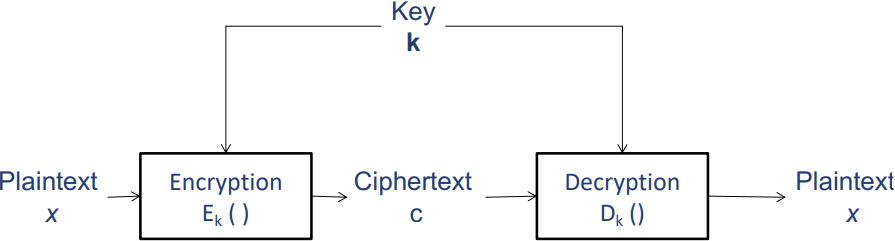
\includegraphics[scale=0.5]{images/cipherdiagram.png} 
There are 2 requirements:
\begin{itemize}
    \item \textbf{Correctness:} For any plaintext: x, key: k, D$_k$(E$_k$(x)) = x. It also must be secure. Formal formulation of security is difficult.
    \item \textbf{Security: } Given a ciphertext, it should be computationally difficult to derive useful information about the key k and plaintext x. The ciphertext should resemble a random sequence of bytes.
\end{itemize}

\subsubsection*{Attack Models: Adversary's Capabilites}
If attacker wants to find the key $\rightarrow$\ \textbf{\textit{total break}}. However attacker may be satisfy a \textbf{\textit{partial break}}.
\begin{itemize}
    \item \textbf{Ciphertext only attack:} adversary is given a collection of a ciphertext \underline{c}, they may know some properties of the plaintext (e.g. plaintext is an english sentence).
    \item \textbf{Known plaintext attack:} adversary is given a collection of plaintext \underline{m} and corresponding ciphertext \underbar{c}, can be used to guess the key and further decrypt other ciphertexts.
    \item \textbf{Chosen plaintext attack (CPA):} adversary has access to a blackbox (an \textit{oracle}). They may choose and feed any plaintext \underline{m} to the blackbox and obtain the corresponding ciphertext a reasonably large number of times \underline{c} (all encrypted with the same key).
    \item \textbf{Chosen cipher attack CCA2:} same as chosen plaintext attack, but the adversary chooses the ciphertext and the blackbox outputs the plaintext. 
\end{itemize}
Indistinguishability (IND) The attacker may satisfy with distinguishability of ciphertext:
with some “non-negligible” probability more than ½, the attacker is able to distinguish
the ciphertexts of a given plaintext (say, “Y”) from the ciphertext of another given
plaintext (say, “N”).

\subsection*{Classical Ciphers}
\subsubsection*{Substitution Cipher}
Plaintext and ciphertext: 
\begin{itemize} 
    \item a string over a set of symbols U. 
    \item Let U= \{ "a", "b", "c" \ldots , "z", "\_" \}
    \item Plaintext may be "hello\_world"
\end{itemize}
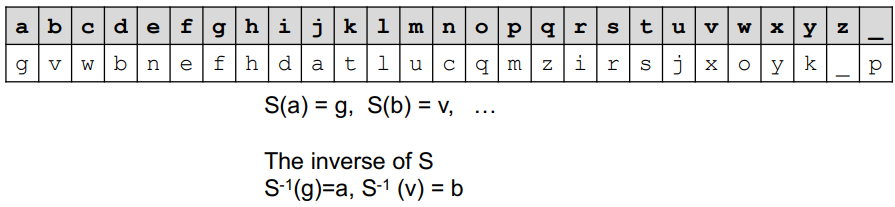
\includegraphics[scale=0.53]{images/substitioncipher.png} 
The key space is the set of all possible keys. The key space size or size of
key space is the total number of possible keys. The key size or key
length is the number of bits required to represent a key. Here, the key
space size is (27!) key size is approximately 94 bits.

\subsubsection*{Attacking Substitution Cipher}
The goal for attackers is to figure out the key. If the key can be found, then the plaintext can be obtained. 
The converse is also true. If the attacker can get information on the plaintext or even the complete plaintext, 
they can also easily obtain the key.
\\

Hence there are 2 levels of access to information:
\begin{itemize}
    \item \textbf{ciphertext only} -- large number of ciphertexts all encrypted using the same key 
    \item \textbf{plaintext} pairs of ciphertext and the corresponding plaintext
\end{itemize}

\textbf{Known Plaintext Attack: Substitution Cipher:} \\
This attack occurs when the attacker has access to pairs of ciphertexts and their corresponding plaintexts. Attacker can 
figure out the entries in the key that are used in both ciphertext and plaintext. With a sufficiently long ciphertext, the
entire key can be determined. If the adversary can derive the key, we call the scheme \textbf{"insecure under known plaintext attack"} or 
\textbf{"broken undder known plaintext attack"}.
\newline

\textbf{First Few Bytes} \\
Not unreasonable for attacker to obtain at least one pair of ciphertext and plaintext as only a small number of bytes is required.
Some of the following can be guessed directly:
\begin{itemize}
    \item Email data: e.g. certain headers or words are fixed ("From", "Subject" \ldots)
    \item Network Protocols: similar to email, as they have fixed headers.
\end{itemize}

\subsubsection*{Exhaustive Search -- Brute Force}
\begin{itemize}
    \item Assume attacker knows a ciphertext \underline{C} and the corresponding plaintext \underline{X}.
    \item For S in all possible substition tables: \\ \ \ \ \ Compute X' = D$_S$(C), if X' == X: break
    \item Since a key in the above table can be represented by a sequence of 27 symbols, size of the key space is 27!
\end{itemize}

\subsubsection*{Frequency Analysis}
Suppose the plaintexts are English sentences. \textbf{Letter frequency distribution} in english is non-uniform. The adversary is able to guess (given a sufficiently long plaintext) by:
\begin{itemize}
    \item Mapping the frequently-occuring letters in the ciphertext to the frequently-occuring letters of english.
    \item Carry out frequency analysis.
\end{itemize}

$\star$\ Substitution cipher is \textbf{not secure under ciphertext-only attack} either.

\subsection*{Permutation Cipher -- transposition cipher}
The encryption first groups the plaintext into blocks of \underline{t} characters, and the applied a secret “permutation” to each 
block by shuffling the characters. The key is the secret “permutation”, which is an 1-1 onto function \textit{e} from
{1,2,..,t} to {1,2,...,t}. The size \underline{t} could be part of the key, that is, \underline{t} is also kept
secret. We can write the permutation \underline{p} as a sequence 
\begin{equation}
    \underline{p} = (p_1, p_2, p_3, \ldots, p_t)
\end{equation}
which shift the character at position \underline{i} to the position \underline{p$_i$} \newline
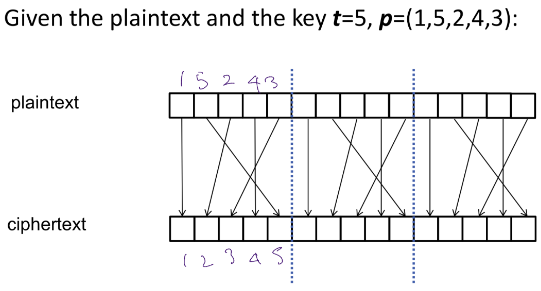
\includegraphics[scale=0.8]{images/permutationcipher.png} \newline
$\star$\ Permutation cipher fails miserably under known-plaintext attack. Given a plaintext and a ciphertext, it is very 
easy to determine the secret key. Permutation cipher is also easily broken under ciphertext only attack if the plaintext 
is English text

\subsection*{One-Time Pad}
Given an \textit{n-bit} plaintext (x$_1$ x$_2$ \ldots x$_n$) and an \textit{n-bit} key (k$_1$ k$_2$ \ldots k$_n$) we can output the ciphertext, C:
\begin{equation}
    C = (x_1 \oplus k_1)(x_2 \oplus k_2)\ldots (x_n \oplus k_n) 
\end{equation}
The condition is that the key and the plaintext must be of the same length. We can then decrypt the ciphertext by XORing the cipher with the
key once more to get the plaintext X:
\begin{equation}
    X = (c_1 \oplus k_1)(c_2 \oplus k_2)\ldots (c_n \oplus k_n) 
\end{equation}

For this to work, we need to be able to transfer the key securely! 

\subsubsection*{What is $\oplus$\ or XOR?}
\begin{itemize}
    \item Commutative: A $\oplus$\ B = B $\oplus$\ A
    \item Associative: A $\oplus$\ (B $\oplus$\ C) = (A $\oplus$\ B) $\oplus$\ C
    \item Identity element: A $\oplus$\ 0 = A, where 0 is the \textit{identity element}
    \item Self-inverse: A $\oplus$\ A = 0
\end{itemize}

$\star$\ From a pair of ciphertext + plaintext, attack can derive the key, but since it is only used one time, this key is useless.
One-time pad leaks no information of the plaintext, even if the attacker has arbitrary running time.

\subsubsection*{Perfect Secrecy}
Attacker's prior knowledge of the unknown plaintext will not change even after they have seen the ciphertext y. Meaning the chances that
the attacker correctly  predicts x before knowing y, and after knowing y, are the same. \newline
\underline{Definition:} A crypto system has \textbf{\textit{perfect secreccy}} if for any distribution of X, for all x, y: 
\begin{subequations}
    \begin{center}
        \framebox{Pr (X = x | Y = y) = Pr(X = x)} 
    \end{center}
\end{subequations}

\subsection*{Modern Ciphers}
Designs of modern ciphers take into consideration of known-plaintext attack, frequency analysis and other known attacks
\begin{itemize}[noitemsep,wide=0pt, leftmargin=\dimexpr\labelwidth + 2\labelsep\relax]
    \item DES (Data Encryption Standard, 1977) $\rightarrow$ Key length too short
    \item RC4 (Rivest's Cipher 4, 1987) $\rightarrow$ Broken in some adoptions
    \item A5/1 (used in GSM, 1987) 
    \item AES (Advanced Encryption Standard, 2001)
\end{itemize}

\subsubsection*{Exhaustive Search, Key Length and Work Factor}
If the key length is 32 bits, there are 2$^{32}$ possible keys. Hence,
the exhaustive search needs to “loop” for 2$^{32}$ times in the worst
case. \newline

We can quantify the security of an encryption scheme by the
length of the key. Consider a scheme \textbf{A} with 64-bit keys and a
scheme \textbf{B} with 54-bit keys. Scheme \textbf{A} is more secure w.r.t.
exhaustive search. \newline

\textbf{DES - Data Encryption Standard} \\
Key length of DES is 56 bits (intentionally short key size). While exhaustive search on 56 bits seemed infeasible in the 70s,
very soon, it is possible using distributed computing or a specialized chip. \newline

\textbf{AES - Advanced Encryption Scheme} \\ 
AES has a block length of 128, and key length can be 128, 192, or 256 bits. It is a symmetric block cipher developed
comprising of the following: Byte Sub, Shift Row, Mix Columns, Add Round key all repeated \textit{n} times.

\subsection*{Block cipher \& Mode-of-Operations}
For a large plaintext, it is divided into blocks (of equal size) before the block cipher
is applied. DES and AES are also known as “Block Cipher”. Block cipher
are designed for some fixed size input/output. \newline

\subsubsection*{ECB Mode - Electronic Code Book}
ECB divides the plaintext into blocks and then applies block
cipher to each block, all with the same key. \newline
$\rightarrow$ BUT, \underline{ECB leaks information!!!}

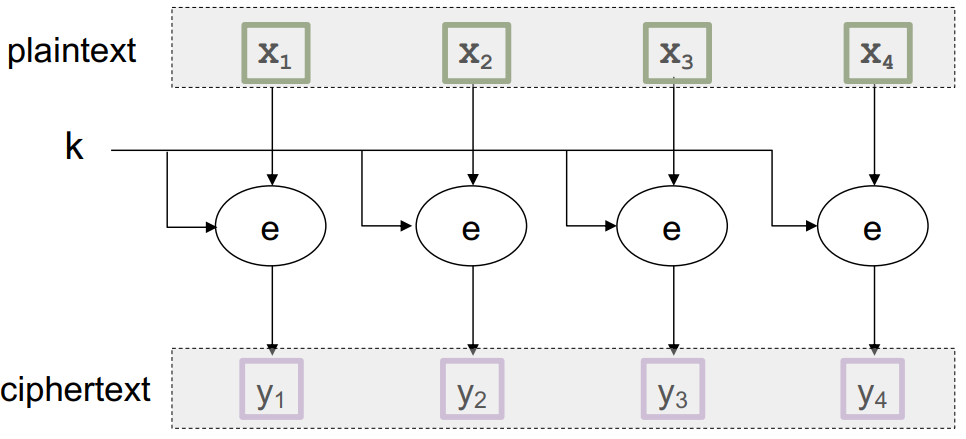
\includegraphics[scale=0.5]{images/ecb.png} 

\begin{center}
    \framebox{\parbox{\dimexpr\linewidth-2\fboxsep-2\fboxrule}{% 
        $\star$ An encryption scheme is \underline{“deterministic”} in the sense that, the encryption algorithm will always produce the same
        output (i.e the ciphertext) when given the same input (i.e. the key and plaintext). \newline
        $\star$ In contrast, a \underline{“probabilistic”} encryption scheme produces different ciphertext even with the same input (key, plaintext).
    }}
\end{center} 

Image below is divided into blocks, and encrypted with some
deterministic encryption scheme* using the same key. Since it is deterministic, any
two blocks that are the same (for e.g. blocks in the white background) will be
encrypted to the same ciphertext.
\begin{center}
    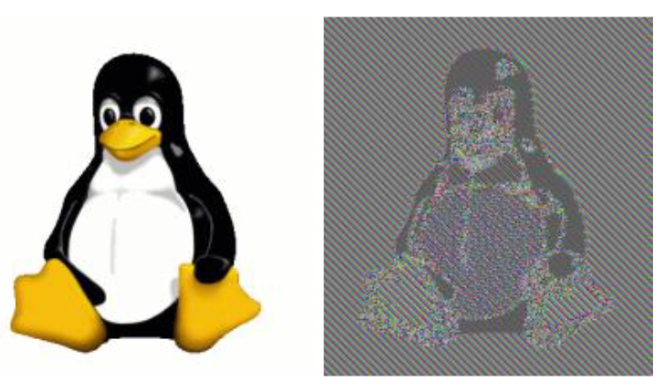
\includegraphics[scale=0.5]{images/penguin.png} 
\end{center}

To prevent leakages of information, there are the following solutions:
\begin{itemize}[noitemsep,wide=0pt, leftmargin=\dimexpr\labelwidth + 2\labelsep\relax]
    \item Use a separate IV for each block (CBC mode) $\rightarrow$ less adopted as final ciphertext would be twice that of plaintext.
    \item Linking of 2 blocks such that upon the encryption of one, we would use that to XOR for the next block.
    \item CTR (Counter) mode, used as a stream cipher.
\end{itemize}

\subsubsection*{CBC - Cipher Block Chaining on AES (mode-of-op)}
The Initial Value (IV) is an arbitrary value chosen during encryption. (different in different encryptions of the same plaintext) $\rightarrow$
\begin{subequations}
    \framebox{y$_0$ = IV, y$_i$ = E$_k$(x$_i$ $\oplus$ y$_{i-1}$)  for i $>$ 0} 
\end{subequations}

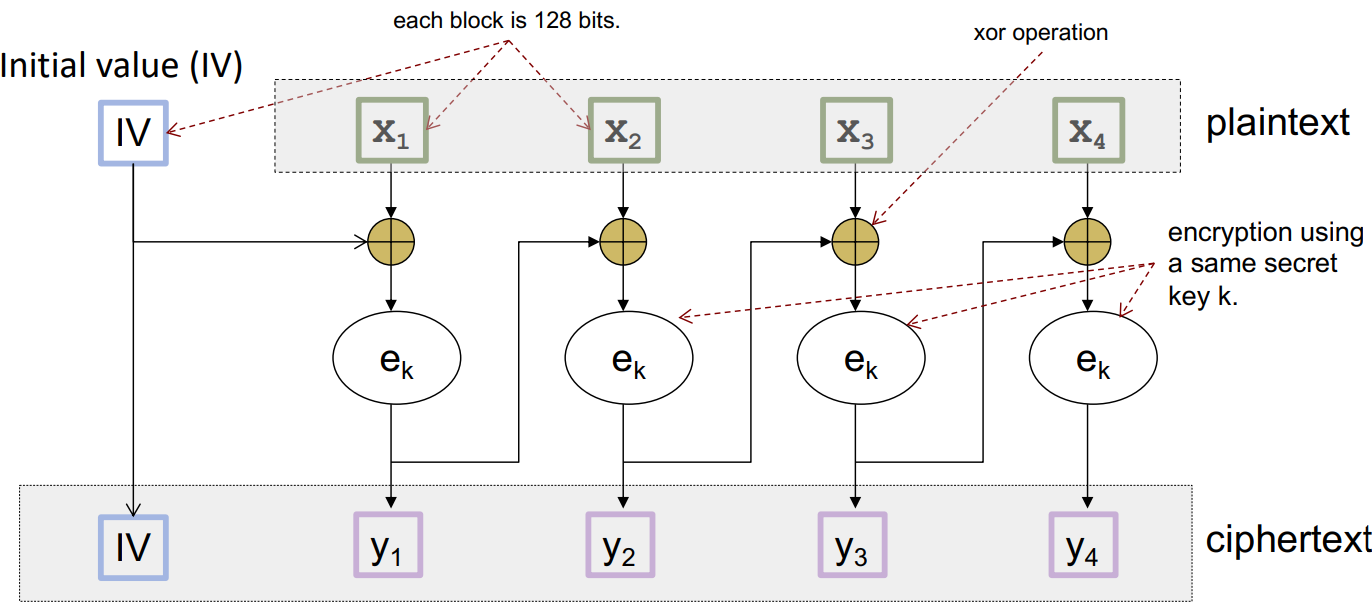
\includegraphics[scale=0.34]{images/cipherblockchaining.png} 


\subsubsection*{CTR - Counter Mode on AES (mode-of-op)}
Type of Stream Cipher.
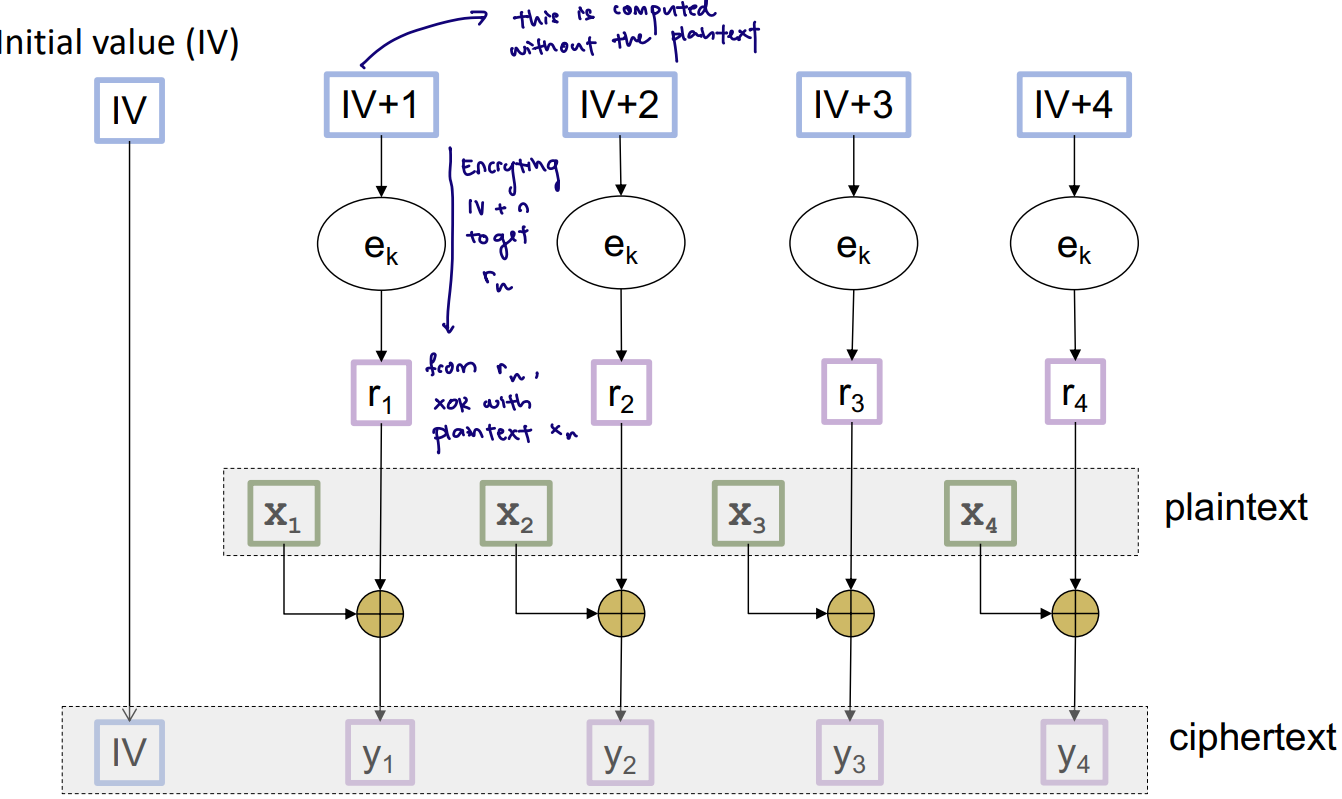
\includegraphics[scale=0.34]{images/countermode.png} 

\subsubsection*{GCM mode - Galois/Counter (mode-of-op)}
It is an authenticated-encryption, ciphertext consists of
an extra tag for authentication. Secure in presence of decryption oracle.

\end{multicols*}

\begin{multicols*}{3}
\subsection*{Stream Ciphers}
Inspired by one-time-pad. Suppose the plaintext is 2$^{20}$ bits, but the secret key is only 256 bits. Stream
cipher generates a 2$^{20}$-bit sequence from the key and treats the generated
sequence as the secret key in one-time-pad. The generator must be
carefully designed, so that it gives \textbf{cryptographically secure pseudorandom
sequence}.

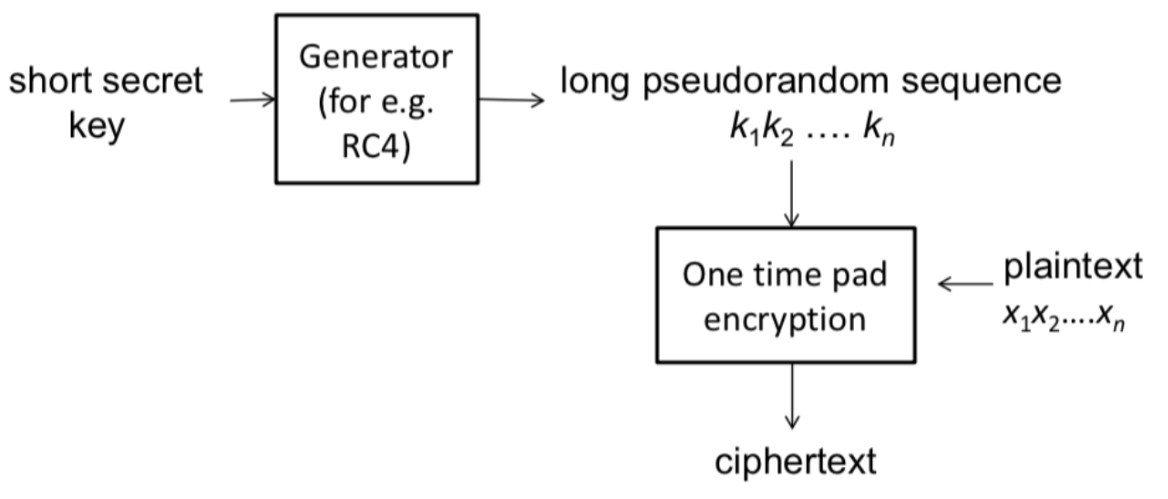
\includegraphics[scale=0.42]{images/streamcipher.png} 

\subsubsection*{Initialization Vector (IV)}
Most ciphers have an IV, which can be randomly chosen or from a counter.
\begin{itemize}[noitemsep,wide=0pt, leftmargin=\dimexpr\labelwidth + 2\labelsep\relax]
    \item \textbf{Encryption:} Long pseudorandom sequence generated from: secret \underline{key + IV}.
    Final ciphertext contains the IV followed by the output of the one-time-pad encryption
    \item \textbf{Decryption:} IV extracted from ciphertext. Plaintext can be obtained by: getting the same
    pseudorandom sequence generated from \underline{key + IV}.
\end{itemize}
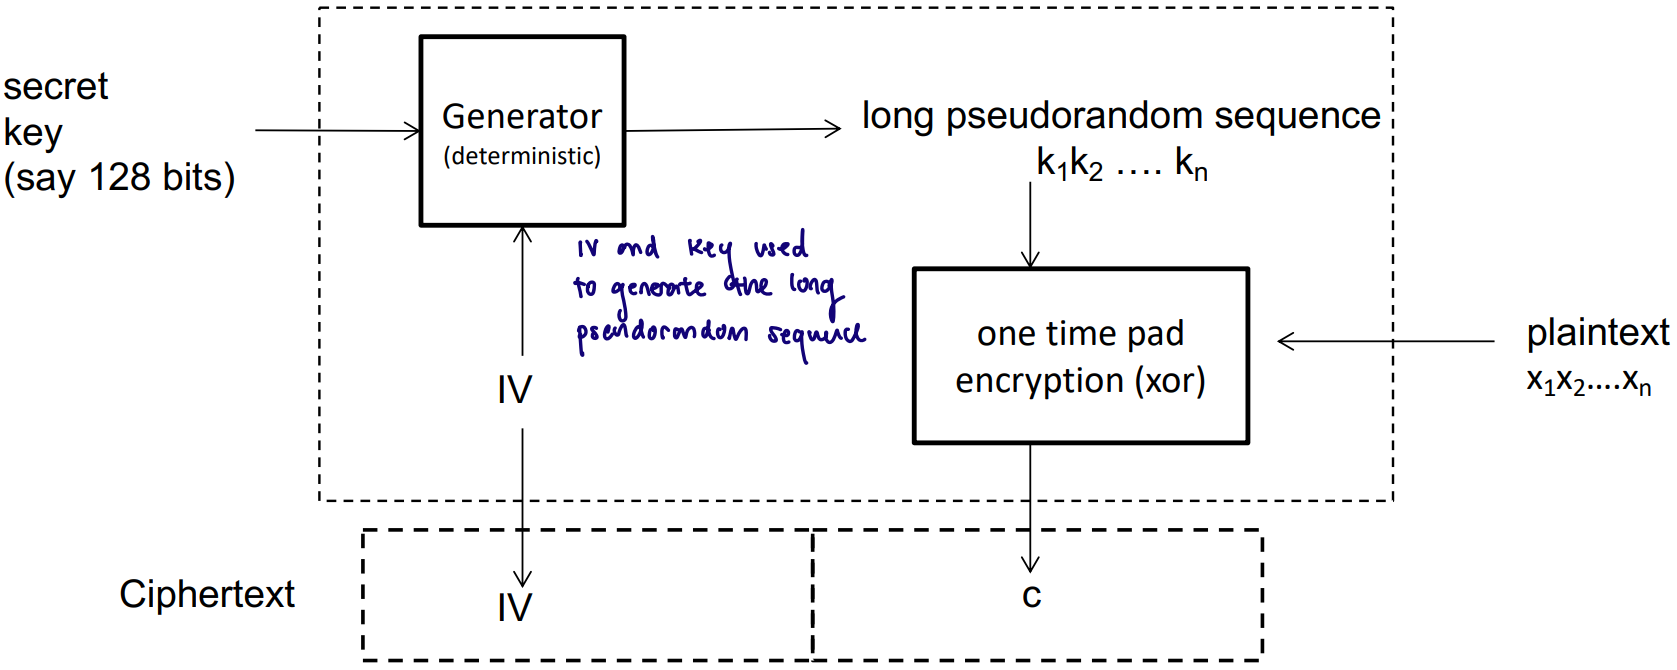
\includegraphics[scale=0.29]{images/initializationvector.png} 

\subsubsection*{Why must we use IV for Stream Ciphers?}
Without the IV, if an attacker can obtain two ciphertexts, they can simply XOR the 2 ciphertexts together. 
Let's say we have ciphertext \textit{U} \& \textit{V}, which are obtained from plaintexts X and Y respectively without using IV.
\begin{subequations}
    \begin{center}
        \framebox{U$\oplus$V = (X$\oplus$K) $\oplus$ (Y$\oplus$K) = (X$\oplus$Y) $\oplus$ (K$\oplus$K) = \underline{(X$\oplus$Y)} } 
    \end{center}
    The above is obtained after doing some manipulation as a result of the associative and commutative properties
    of XOR = X$\oplus$Y.
\end{subequations}

Let us take X and Y as black and white images, where every pixel corresponds to a bit.

\begin{center}
    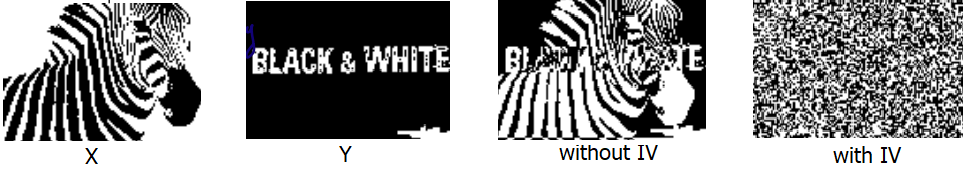
\includegraphics[scale=0.5]{images/initializationvectorimportance.png} 
\end{center}

They look different because K$_1$ and K$_2$ are different due to it being produced
by different IVs, thus there is no cancelling out when XOR both images. IV makes an 
encryption \underline{probabilistic}

\section*{Triple DES}
DES not secure w.r.t. today computing power. We can improve it by encrypting multiple times $\rightarrow$ using different keys. 
DES doesn’t form a group in the sense that, E$_{k1}$(E$_{k2}$(x)) is not the same
as E$_{k3}$(x) for some \textit{k3}.

\subsection*{Meet-in-the-middle Attack}
\textit{Known plaintext attack}, where the attacker's goal is to find the keys \textit{k1} and \textit{k2}.
\begin{itemize}
    \item Compute two sets of \textbf{\textit{C}} and \textbf{\textit{M}}. \textbf{\textit{C}} contains ciphertexts of
        \textbf{\textit{m}} encrypted with all possible keys. \textbf{\textit{M}} contains plaintexts of \textbf{\textit{c}} 
        decrypted with all possible keys.
    \item Find common element \textbf{\textit{C}} and \textbf{\textit{M}}, thereby obtaining both keys.
    \item In general, for \textit{k-bit} keys, it reduces the number 
        of crypto operations to 2$^{k+1}$ using approx 2$^{k+1}$ units of storage space.
\end{itemize}

\includegraphics*[scale=0.27]{images/meetinthemiddle.png}
\begin{center}
    \framebox{\parbox{\dimexpr\linewidth-2\fboxsep-2\fboxrule}{% 
        $\star$ Remedy -- Use Triple Encryption, but with 2 keys. Both below believed to have the same level of security:
        \begin{itemize}
            \item E$_{k1}$(E$_{k2}$(E$_{k1}$( x )))
            \item OR E$_{k2}$(E$_{k1}$(E$_{k2}$( x )))
        \end{itemize}
    }}
\end{center} 

\subsection*{Padding Oracle Attack}
Attacker has a ciphertext including (IV, c) and access to a \underline{padding oracle}.
Attacker's goal is to get the plaintext of (IV, c) The cipher text is encrypted with a
secret key \textit{k} and the oracle knows \textit{k}.

\subsubsection*{Padding - PKCS\#7}
Suppose a block size is 8 bytes, and the last block has 5 bytes only (thus 3 extra bytes required),
the padding will be done as follows (if the last block is full, an extra block of all zeroes are added.):
\begin{multicols*}{2}
    \framebox{\parbox{\dimexpr\linewidth-2\fboxsep-2\fboxrule}{% 
        \scriptsize{DD DD DD DD DD DD DD DD}
    }}
    \framebox{\parbox{\dimexpr\linewidth-2\fboxsep-2\fboxrule}{% 
        \scriptsize{DD DD DD DD DD 03 03 03}
    }}
\end{multicols*}

Padding oracle attack takes advantage of the deterministic natrue of a Block Cipher, if the
plaintext is unchanged, the resultant ciphertext (and vice versa) would also remain the same.
Padding oracle attack also takes advantage of XOR operations:
\framebox{\parbox{\dimexpr\linewidth-2\fboxsep-2\fboxrule}{% 
    for any A, B, C if A $\oplus$ B = C, B $\oplus$ C = A, then A $\oplus$ C = B.
}}

\subsection*{Padding Oracle Attack - Example (on CBC)}
Suppose the attacker wants to find out what is \textit{t$_2$}. 
\begin{itemize}
    \item First, force the plaintext to have a padding of 2 (02 02) -- allow reverse engineering of the XOR operation to find out the original plaintext in that byte position
    \item Next, use exhaustive search to find out which values of \textit{t$_2$} from the previous block together with the ciphertext from block C2, when XORed, will produce a "YES" from the padding oracle.
    \begin{itemize}
        \item If "NO", repeat exhaustive search.
        \item If "YES", this means that the padding is correct, and that means this value of \textit{t$_2$} is the correct value for that byte.
    \end{itemize}
    \item Finally, we XOR the value \textit{t$_2$} with that of the ciphertext from P2 to obtain the intemediary \textit{x$_2$}.
    \item From the intemediary, we can use the unchanged key we already know to get the \underline{original plaintext}.
\end{itemize}
\includegraphics*[scale=0.38]{images/paddingoracleattack.png}
  
\section*{Cryptography Pitfalls}
\subsection*{Wrong choices of IV}
Some applications overlooked IV generation. As a result, under some situations, the same IV is reused.
\begin{itemize}
    \item e.g. To encrypt a file F, the IV is derived from the filename. It
    is quite common to have files with the same filename $\rightarrow$ Schneier on Security, Microsoft RC4 Flaw:
        \begin{itemize}[noitemsep,wide=0pt, leftmargin=\dimexpr\labelwidth + 2\labelsep\relax]
            \item The stream cipher RC4 with key length up to 128 bits is used in Microsoft Word and Excel to protect
            documentss. But when an encrypted document gets modified and saved, the initialization vector remains the same,
            thus the same keystream generated from RC4 is applied to encrypt different versions of that document.
        \end{itemize}
    \item When using AES under the “CBC mode”, the IV should be unpredictable in order to prevent a certain type of attack.
    (So, it is vulnerable to choose IV as 1,2,3,....)
    \begin{itemize}[noitemsep,wide=0pt, leftmargin=\dimexpr\labelwidth + 2\labelsep\relax]
        \item The Browser Exploit Against SSL/TLS Attack (BEAST) exploits this, as when encrypting multiple packets, the IV
        of a packet would be the last ciphertext block of the previous packet, which is visible to anyone.
    \end{itemize}
\end{itemize}

\subsection*{Reusing One-Time-Pad Key}
Similar to reusing IV, if the one-time-pad key is reused and attacker notices it, it is possible to decrypt entire messages. Project
Venona saw the decryption of encrypted messages from the Soviet Union by the US.

\subsection*{Predictable Secret Key Generation}
When progamming, we may use packages such as \verb|java.util.Random| despite the fact that it is not actually secure. 
\verb|java.security.SecureRandom| is preffered because:

\begin{itemize}[noitemsep,wide=0pt, leftmargin=\dimexpr\labelwidth + 2\labelsep\relax]
    \item \textbf{Size:} \verb|Random| class only has 48 bits, whereas \verb|SecureRandom|, can have up to 128 bits, smaller chance of repeated \verb|SecureRandom|.
    \item \textbf{Seed Generation:} \verb|Random| uses system clock to generated the seed, attacker can easily replicate if they know when the seed was produced. \verb|SecureRandom|
    takes random data from OS as most OSes collect and store these data in files (interval between keystrokes etc.) and use that as the seed
    \item \textbf{Breaking the code:} \verb|Random| requries 2$^{48}$ tries (practically possible with compute resources today), \verb|SecureRandom| requires 2$^{128}$ attemps, may take many years.
    \item \textbf{Generating Function:} Standard Oracle JDK 7 implementation uses a Linear Congruential Generator to produce random values in 
    \verb|java.util.Random|. \verb|java.security/SecureRandom| implements SHA1PRNG algorithm, using SHA1 to generate pseudorandom numbers.
    \item \textbf{Security:} \verb|java.util.Random| must not be used for either security-critical applications/protecting sensitive data.
\end{itemize}

\subsubsection*{Designing your own crypto/cipher}
Don’t design your own crypto, or even make slight
modification to existing scheme... unless you have in-depth
knowledge on the topic.

\subsection*{Kerckhoffs’s principle}
A system should be secure even if everything about the system,
except the secret key, is public knowledge. 
\subsubsection*{Arguments \underline{against} obscurity}
\begin{itemize}[noitemsep,wide=0pt, leftmargin=\dimexpr\labelwidth + 2\labelsep\relax]
    \item RC4 introduced in 1987 with its algorithm as a trade secret. In 1994, a description of its algorithm was
    anonymously posted in a mailing group.
    \item MIFARE Classic is a contactless smartcard widely used in Europe. It uses a set of proprietary protocols/algorithms. However, they are reverse-engineered in 2007. It turns out
    that the encryption algorithms are already known to be weak (with 48-bit keys) and breakable.
\end{itemize}

\subsection*{Security through Obscurity}
To hide the design of the system in order to achieve security. 
\begin{itemize}[noitemsep,wide=0pt, leftmargin=\dimexpr\labelwidth + 2\labelsep\relax]
    \item obscurity can be used as an addition layer in the \textbf{defense-in-depth}
    strategy.
    \item NOT advisable to reveal the computer network structure and settings (for example,
    location of firewall and the firewall rules), although these are not “secrets”.
    \item Although it is advisable to make the algorithm public, it is not advisable to publish the
    actual program used in a smart-card. By publishing the program/code, advisory may
    able to identity implementation flaw that was previously unaware of, or carry out
    side-channel attacks. 
    \item Usernames are not secret. However, it is not advisable to publish all the usernames
\end{itemize}

\section*{\underline{Authentication (Password)}}
Authentication: The process of assuring that the communicating
entity, or origin of a piece of information, is the one that it claims to
be. \\ 

There are 2 types of authentication:

\begin{enumerate}[noitemsep,wide=0pt, leftmargin=\dimexpr\labelwidth + 2\labelsep\relax]
    \item \textbf{Entity authentication:}
        \begin{itemize}[noitemsep,wide=0pt, leftmargin=\dimexpr\labelwidth + 2\labelsep\relax]
            \item For connection-oriented communication
            \item Verifying authenticity of entities involved in a connection
            \item Mechanisms: password, challenge and response, cryptographic protocol
        \end{itemize}
    \item \textbf{Data-origin authentication:}
        \begin{itemize}[noitemsep,wide=0pt, leftmargin=\dimexpr\labelwidth + 2\labelsep\relax]
            \item For connectionless communication
            \item Verifying the origin of a piece of information
            \item Mechanisms: Crypto primitives such as MAC or digital signature. 
        \end{itemize}
\end{enumerate}
\subsection*{Authenticity vs Integrity}
Authentic is an adjective to say that the claimed enity/origin is assured by supporting evidence. 
Authenticity is the condition of being authentic. 

Authenticity and integrity are thus related. In the context of an insecure channel, we can say that 
a message that has been modified in transit means that it no longer comes from its original source. 

In other words, a message whose integrity is compromised also means that its authenticity is compromised.
As such \textbf{data-origin authenticity implies data integrity}. But \textbf{data integrity does not imply}
\textbf{data-origin authenticity}. Authenticity is thus a stronger requirement than integrity.

\subsection*{Password System}
A password is part of an authentication system that usually consists of:
\begin{itemize}[noitemsep,wide=0pt, leftmargin=\dimexpr\labelwidth + 2\labelsep\relax]
    \item Identity (Identification): need not be kept secret. It can be a username in a system, bank account number, customer ID etc.
    \item Password (Authentication): password is kept secret, only the authentic user \& server knows it. The fact that an entity knows the password \textbf{implies that it is either the server or the authentic user.}
\end{itemize}
\begin{enumerate}[noitemsep,wide=0pt, leftmargin=\dimexpr\labelwidth + 2\labelsep\relax]
    \item \textit{Bootstrapping}
        \begin{itemize}[noitemsep,wide=0pt, leftmargin=\dimexpr\labelwidth + 2\labelsep\relax]
            \item Password is to be established during Bootstrapping, done by:
            \begin{itemize}[noitemsep,wide=0pt, leftmargin=\dimexpr\labelwidth + 2\labelsep\relax]
                \item Server/user chooses a password and sends it to the user/server through another communication channel.
                \item Default password.
            \end{itemize}
        \end{itemize}
    \item \textit{Password Authentication}
        \begin{itemize}[noitemsep,wide=0pt, leftmargin=\dimexpr\labelwidth + 2\labelsep\relax]
            \item Protocol: \framebox{\parbox{\dimexpr\linewidth-2\fboxsep-2\fboxrule}{% 
                User $\rightarrow$ Server: My name is \textbf{Alice} \newline
                Server $\rightarrow$ User: What is your password  \newline
                User $\rightarrow$ Server: \textbf{OpenSesame} \newline
                Server verifies whether password is correct.
            }} \newline
            \item Authentication can also be carried out without interactions: \newline
            User sends sms to server:
            UserId: \textbf{Alice@nus.edu.sg} Password: \textbf{OpenSesame}. Instructions: Unsubscribe from your mailing list. No more junk mail.
            \item This protocol is \textbf{"weak authentication"}, subjected to replay attack (packet sniffing/eavesdropper in communcation channel).
        \end{itemize}
    \item \textit{Password reset}
        \begin{itemize}[noitemsep,wide=0pt, leftmargin=\dimexpr\labelwidth + 2\labelsep\relax]
            \item Only authorized entities can reset the password. How do we verify the entity is authentic?
            \item Need to authenticate entity before allowing entity to change password
        \end{itemize}
\end{enumerate}

\subsection*{Attacks on the Password System}
Attacker may intercept the password during bootstrapping. They can also target the use of default passwords (e.g. IP Security Cameras). 
\textbf{No individual passwords:} Cost increase for device manufacturer, print passwords on each equipment/manual/case.

\subsection*{Searching for the Password}
\subsubsection*{Dictionary Attack}
Ability to test $\rightarrow$ feed a guess into login screen:
\begin{itemize}[noitemsep,wide=0pt, leftmargin=\dimexpr\labelwidth + 2\labelsep\relax]
    \item \textbf{Exhaustive search} test all combinations to guess passwords
    \item \textbf{Dictionary attack} tests passwords stored in a "dictionary" (contain words from English dictionary, known compromised passwords, most passwords are generated by Humans).
    \item Dictionary attack could also exhaustively test combinations of words in dictionary. Exhaustively try all possible capitalization of words ("a" substitute by "@").
\end{itemize}
Two scenarios in dictionary attacks:
\begin{itemize}
    \item \textbf{Online dictionary} attack: an attacker must interact with the authentication system during the searching process. (attacker must be online)
    \item \textbf{Offline dictionary} attack: There are 2 phases
        \begin{enumerate}[noitemsep,wide=0pt, leftmargin=\dimexpr\labelwidth + 2\labelsep\relax]
            \item Attacker obtains some information \textbf{D} about password (sniff hash from interactions, or steal password file).
            \item Next, attacker carries out the searches using \textbf{D} without interacting with the system.
        \end{enumerate}
\end{itemize}

\subsubsection*{Guessing the password from social information}
Attacker gathers social information about user to guess password. 

\subsection*{Stealing the password}
\subsubsection*{Sniffing}
Shoulder sniffing (look-over-the shoulder), or \textbf{Sniffing the communication}, not as common now, some older systems
sent passwords over public network (not encrypted).

\subsubsection*{Viruses, Keylogger}
Key-logger records keystrokes, sends information back to attacker.
\begin{itemize}[noitemsep,wide=0pt, leftmargin=\dimexpr\labelwidth + 2\labelsep\relax]
    \item (software) Some computer viruses are designed as a \textbf{key-logger}
    \item (hardware) Hardware key-logger physically connected to device
\end{itemize}

\subsection*{Phishing}
A type of \textbf{social engineering}. Victim tricked to voluntarily send the password to the attacker. Phishing attacks ask for passwords
under some false pretense. Typically, it tricks the user to visit a website, which is spoofed login page.
\subsubsection*{Spear Phishing}
Phishing can be targeted to a particular small group of users (for example, NUS Staff). These are known as 
\textit{spear phishing} which is an example of \textit{targeted attacks}.

\subsection*{Cache}
Using shared workstation, information keyed in could be cached. Next user still has access to cache.

\subsubsection*{Insider attack}
Malicious system admin steals password file. OR System admin's account compromised, lost of password file.

\subsection*{Preventive Measures}
\subsubsection*{1. User Training:} 
Workshop, reminders. Embedded Phishing Exercise (Authorized entities send out "phishing" emails to employees).
\subsubsection*{2. Blacklisting}
Repository site keeps list of phishing site, blacklisted by browser or firewall.
\subsubsection*{3. Using Strong Password}
Truly random password, using automated password generator. High "Entropy" difficult to remember.
\begin{itemize}[noitemsep,wide=0pt, leftmargin=\dimexpr\labelwidth + 2\labelsep\relax]
    \item User selection:
        \begin{itemize}[noitemsep,wide=0pt, leftmargin=\dimexpr\labelwidth + 2\labelsep\relax]
            \item Mnemonic Method: \underline{Pbmbval!}
            \item Altered Passphrases: \underline{Dressed*2*tge*9z}
            \item Combining/Altering Word: \underline{B@nkC@mera}
        \end{itemize}
    \item Usability: Strong passwords are difficult to remember. Difficult to enter alphanumeric passwords on mobile devices.
\end{itemize}
\subsubsection*{3a. Password Ageing}
Recommended for users to regularly change passwords. 
\subsubsection*{Online vs Offline Attack}
\begin{itemize}[noitemsep,wide=0pt, leftmargin=\dimexpr\labelwidth + 2\labelsep\relax]
    \item \textbf{Online:} To check whether a password is correct, the attacker needs to
    communicate with a server not under his control. E.g.
    - Attacker obtained a list of 1000 valid nusnet id, to find the
    password for some of them. The attacker writes an automated script that attempt to
    login to Canvas using guessed passwords for each of these 1000 valid nusnet id.
    \item \textbf{Offline:} To check whether a password is correct, the attacker can
    execute some algorithm without connecting to a server. \\
    - Attacker has an AES encrypted pdf file. The key is derived from a password. The
    attacker wants to find the password. \\
    - In some password authentication protocols, a “hash” of the password is sent in clear.
    The attacker first obtained the hash by eavesdropping a valid login session. Next, the
    attacker went offline and searched for the password. WPA2 personal is vulnerable to
    this form of offline dictionary attack.
\end{itemize}



\subsection*{Enhancing Password System}
\begin{itemize}[noitemsep,wide=0pt, leftmargin=\dimexpr\labelwidth + 2\labelsep\relax]
    \item Online dictionary attacks more difficult, there may be intentional delay into login sessions or account locking after a few failed attempts.
    \item Offline dictionary attacks more difficult, KDF applied to password, forces intensive computation, but has delay during legitimate usage.
\end{itemize}

\subsection*{Additional Protection to password files}
During authentication, password entered by entity is hashed, then compared with value stored in password file.
To verify whether password \textbf{P} belongs to a user \textbf{U}:
\begin{enumerate}[noitemsep,wide=0pt, leftmargin=\dimexpr\labelwidth + 2\labelsep\relax]
    \item Compute d = Hash(\textbf{P})
    \item If <\textbf{U}, d> is in the password file, accept, else reject.
\end{enumerate}
We cannot have the same password being hashed to the same value for 2 different usernames. Allows attackers to obtain all un-hashed passwords of the same value
simply by comparing hashed values. To prevent this, we add a \textbf{salt}: random string of characters to the front of the password before hashing. Salt randomly generated for all users, stored in password file.

\subsection*{Self-help Password Reset}
\subsubsection*{1. Security Question}
Security-Cost-Usability Tradeoff: viewed as a mechansim for \textbf{fallback authentication}
\begin{itemize}[noitemsep,wide=0pt, leftmargin=\dimexpr\labelwidth + 2\labelsep\relax]
    \item Enhance usability: user can still login if password is lost
    \item Reduce cost: reduces oeprating cost of helpdesk
    \item Weak security: attackers have another mean to obtain access
\end{itemize}
\subsubsection*{2. Recovering email's account}
\framebox{\parbox{\dimexpr\linewidth-2\fboxsep-2\fboxrule}{% 
    \begin{enumerate}
        \item User $\rightarrow$ System: User id is \underline{X}, I want to reset
        \item System $\rightarrow$ User: Send email to user, URL contains an OTP 
        \item User $\rightarrow$ System: OTP is \underline{OTP1}, This is my new password
        \item System checks if OTP correct, if correct, reset
    \end{enumerate}
}}

\subsection*{ATM Skimmer}
For authentication, there is a (1) Card and (2) Pin. Card contains magnetic strip, storing user account id, PIN is the password.
AN ATM Skimmer steals victim's account id + password.
\begin{enumerate}
    \item card-reader attached on top of existing ATM reader;
    \item camera overlooking the keypad/spoofed key-pad on top of existing keypad;
    \item means to record/transmit the information back to attacker. 
\end{enumerate}
\subsubsection*{Measures against ATM Skimmers}
\begin{enumerate}[noitemsep,wide=0pt, leftmargin=\dimexpr\labelwidth + 2\labelsep\relax]
    \item Anti-skimmer device: prevents external card reader attachment
    \item Sheilding of keypad
    \item Awareness among users
\end{enumerate}

\section*{Biometric}
\begin{itemize}[noitemsep,wide=0pt, leftmargin=\dimexpr\labelwidth + 2\labelsep\relax]
    \item \textbf{enrollment}, a template of user's biometric data is captured and stored. (same as bootstrapping)
    \item \textbf{verification}, biometric data of person-in question captured and compared with template using matching algorithm (algo decides accept or reject).
\end{itemize}
\includegraphics*[height=3.1cm, width=8.5cm]{images/biometric.png}

There is inevitable noise in capturing biometric data, leading to error in making matching decision.
\textbf{False Match Rate(FMR)} and \textbf{False Non-Match Rate (FNMR)}
\begin{equation}
    FMR = \frac{number \ of \ successful \ false \ matches \ (B)}{number \ of \ attempted \ false \ matches \ (B + D)}
\end{equation}
\begin{equation}
    FNMR = \frac{number \ of \ rejected \ genuine \ matches \ (C)}{number \ of \ attempted \ genuine \ matches \ (A + C)}
\end{equation}
\begin{center}
    \begin{tabular}{ |c|c|c|c| } 
        \hline
        & Accept & Reject\\
        \hline
        \multirow{2}{8em}{Genuine attempt \\ False attempt} & A & C \\ 
        & B & D \\ 
        \hline
    \end{tabular}
\end{center}
\begin{itemize}[noitemsep,wide=0pt, leftmargin=\dimexpr\labelwidth + 2\labelsep\relax]
    \item \textbf{Equal-Error Rate (EER):} FNMR = FMR
    \item \textbf{False-to-enroll Rate (FER):} Some user's biometric data cannot be captured e.g. due to injury.
    \item \textbf{Failure-to-capture (FTC):} User's biometric data may fail to be captured during transactions e.g. dirty fingers.
\end{itemize}
\subsubsection*{Attack of biometric system}
Some biometric data can be easily spoofed. Other systems include \textbf{liveness detection} to verify if the entity being scanned is indeed \underline{live} or instead of something spoofed.

\subsection*{n-Factor Authentication (2FA)}
Require 2 different authentication factors:
\begin{enumerate}[noitemsep,wide=0pt, leftmargin=\dimexpr\labelwidth + 2\labelsep\relax]
    \item Something you know: Password, PIN
    \item Something you have: Security token, mobile phone, ATM Card
    \item Who you are: Biometric
\end{enumerate}

\subsubsection*{OTP Token}
Hardware generates one time password, each token and the server share some secrets. 
\begin{enumerate}[noitemsep,wide=0pt, leftmargin=\dimexpr\labelwidth + 2\labelsep\relax]
    \item \textbf{Time-based:} Based on shared secret and current time interval, generate password \textbf{\textit{K}}.
    \item \textbf{Sequence-based:} An event (user pressing button) triggers change of OTP.
\end{enumerate}

\textbf{Example: Password + SMS} \\
\textbf{Registration:} User gives server mobile phone number and password. \\
\textbf{Authentication:}
\begin{enumerate}[noitemsep,wide=0pt, leftmargin=\dimexpr\labelwidth + 2\labelsep\relax]
    \item User sends password and username to server
    \item Server verifies password is correct, then sends OTP to user through SMS
    \item User receives SMS, enters OTP
    \item Server verifies OTP is correct
\end{enumerate} 

\begin{itemize}[noitemsep,wide=0pt, leftmargin=\dimexpr\labelwidth + 2\labelsep\relax]
    \item OTP generated from a factor.
    \item Password is long term and can be the same for a long duration. OTP is valid for a short period of time/for a specific transaction.
    \item If attack somehow managed to eavesdrop session and steal OTP with password, password can still be used as password + OTP insufficient for replay attacks of further sessions.
    \item OTP does not expose (non-password) factor during authentication. Even if session compromised, confidentiality still preserved. 
\end{itemize}

\section*{\underline{Authenticity}}
\subsubsection*{Public Key Encryption}
Public-key scheme uses different keys for encryption + decryption. \\
Only with the \textbf{private key k$_d$} can we decrypt the ciphertext.
\includegraphics*[scale=0.32]{images/publickeyencryption.png}

\subsubsection*{Security Requirements}
Given the public key and ciphertext (not private key) it is difficult to determine the plaintext.
\newline

ADVANTAGES \\ 
In PKC, if there are multiple entities A$_1$, ... A$_n$ each has their own $\textless$private key, public key$\textgreater$.
Each entity only needs to broadcast their \underline{public key}, keeping private \textit{secret}.
\newline

If we do not use PKC, then any 2 entities must share a symmetric key via a secure channel, requiring both entities to know one another before actual communication.
(PKC still needs a secure broadcast channel to distribute the \textbf{public key}).
\includegraphics*[height=5cm, width=8.5cm]{images/keydistribution.png}

\subsection*{RSA -- Rivest–Shamir–Adleman}
\begin{enumerate}[noitemsep,wide=0pt, leftmargin=\dimexpr\labelwidth + 2\labelsep\relax]
    \item Randomly choose 2 large primes \textbf{p} and \textbf{q}, computes \textbf{n = pq}
    \item Randomly choose encryption exponent \textbf{e}: 
    \noindent\begin{equation*}
        gcd(e, (p-1)(q-1))
    \end{equation*}
    \item Find decryption exponent \textbf{d}, where 
    \noindent\begin{equation*}
        d \ e  \ mod(p-1)(q-1) = 1
    \end{equation*}
    \item Published (\textbf{n}, \textbf{e}) as public key, safe-keeps (\textbf{n}, \textbf{d}) as private key
\end{enumerate}
\begin{equation*}
    \noindent\boxed{
    \begin{array}{rcl}
        n = pq \\
        \phi(n) = (p-1)(q-1) \\
        d = e^{-1} mod \phi(n)
    \end{array}
    }
\end{equation*}
\includegraphics*[height=2.3cm, width=8.5cm]{images/RSA.png}

\textbf{Property of RSA} \\
We can also use the decryption key \textbf{d} to encrypt and encryption key \textbf{e} to decrypt.
This does not hold in other public key schemes. \newline

\textbf{Algorithmic issues}
\begin{itemize}[noitemsep,wide=0pt, leftmargin=\dimexpr\labelwidth + 2\labelsep\relax]
    \item (step 1): How to find random prime? Rnadomly pick a number and test whether it is a prime.
    \item (step 3): Value of \textbf{d} can be efficiently computed from \textbf{e} and \textbf{n} using the Eucildean algorithm.
    \item Encryption of plaintexts at different times give the same ciphertexts. Some form of IV or padding is needed to introduce an extra element of randomness.
\end{itemize}

\subsubsection{Issues that RSA faces}
\underline{POOR EFFICIENCY AND PERFORMANCE}
\begin{itemize}[noitemsep,wide=0pt, leftmargin=\dimexpr\labelwidth + 2\labelsep\relax]
    \item RSA is significantly slower than AES (10,000x slower)
    \item A 128-bit AES has the same key strength as a 3072-bit RSA
\end{itemize}

To overcome this issue: \newline
When a large file is to be encrypted under the public key setting, for efficiency, the
following steps can be carried out:
\begin{enumerate}[noitemsep,wide=0pt, leftmargin=\dimexpr\labelwidth + 2\labelsep\relax]
    \item Randomly choose an AES key k
    \item Encrypt F using AES with k as the key to produce the ciphertext C
    \item Encrypt k using RSA to produce the ciphertext q
    \item The final ciphertext consists of 2 components: (q, C) \newline
\end{enumerate} 

The reverse is to be done for decryption:
\begin{enumerate}[noitemsep,wide=0pt, leftmargin=\dimexpr\labelwidth + 2\labelsep\relax]
    \item Decrypt q using RSA to produce the key k
    \item Decrypt C using AES with k as the key to produce plaintext F
\end{enumerate}
\includegraphics*[height=2.3cm, width=8.5cm]{images/largefilersa.png}

\underline{SECURITY OF RSA} \newline
RSA not necessarily 'more secure' than AES. It can be shown that getting the private key
from public key is as difficult as factorization. Unknown if the problem of
getting the plaintext from ciphertext and public key is as difficult as factorization. \newline

The 'textbook' RSA has to be modified so that difficult encryptions of the same plaintext to lead different
ciphertexts, and such modifications are not straightforward (e.g. PKCS\#1).

\subsection*{Strengths of PKC}
Main strength is the public key setting, allowing the entity in public to perform encryption without a pre-establihed pair-wise secret key.
This secret-key-less feature is also useful in providing authentication. PKC is rarely used to encrypt a large file.

\subsection*{Cryptographic Hash}
A hash is a function that takes in an arbitrarily long message as input and outputs a fixed size \textbf{digest}.

\includegraphics*[height=1.3cm, width=8.5cm]{images/hash.png}

\textbf{Security Requirements:}
\begin{itemize}[noitemsep,wide=0pt, leftmargin=\dimexpr\labelwidth + 2\labelsep\relax]
    \item Preimage Resistant or One-way: Given a digest d, it is difficult to find a m such that h(m) = d. (Difficult to reverse engineer)
    \item Second-preimage resistant: Given m$_1$, difficult to find a second preimage m$_1$ $\ne$ m$_2$ such that h(m$_1$) = h(m$_2$).
    \item Collision-resistant: Difficult to find 2 different menssages m$_1$ $\ne$ m$_2$ that hashes into the same digest (h(m$_1$) = h(m$_2$))
\end{itemize}

\underline{Popular Hashes:} SHA-0, SHA-1, SHA-2, SHA-3
\begin{itemize}
    \item SHA-0 was published by NIST in 1993. It produces a 160-bits digest. It was withdrawn
    shortly after publication and superseded by the revised version SHA-1 in 1995.
    \item SHA-1 is a popular standard. It produces 160-bits message digest. It is employed in SSL,
    SSH, etc.
    \item In 1998, an attack that finds collision of SHA-0 in 261 operations was discovered. (Using
    the straight forward birthday attack, collision can be found in 2160/2 = 280 operations). In
    2004, a collision was found, using 80,000 CPU hours. In 2005, Wang Xiaoyun et al.
    (Shandong University) gave attack that can finds collision in 239 operations.
    \item In 2001, NIST published SHA-224, SHA-256, SHA-384, SHA-512, collectively known as SHA-2.
    The number in the name indicates the digest length. No known attack on full SHA-2 but
    there are known attacks on “partial” SHA-2, for e.g. attack on a 41-rounds SHA-256 (the full
    SHA-256 takes 64 rounds)
    \item In 2005, Xiaoyun Wang et al gave a method of finding collision of SHA-1 using 269
    operations, which was later improved to 263 . A collision was found in 2017. It took 110
    GPU years, completed 263 SHA1 operations.
    \item In Nov 2007, NIST called for proposal of SHA-3. In Oct 2012, NIST announced the winner,
    Keccak (pronounced “catch-ack”). 
\end{itemize}

\underline{Popular but obselete:} MD5
\begin{itemize}
    \item Designed by Rivest. MD, MD2, MD3, MD4, MD5, MD6.
    \item MD6 was submitted to NIST SHA-3 competition but did not advance to the
    second round of the competition.
    \item MD5 was widely used. It produces 128-bit digest.
    \item In 1996, Dobbertin announced a collision of the compress function of MD5.
    \item In 2004, collision was announced by Xiaoyu Wang et al. The attack was reported
    to take one hour.
    \item In 2006, Klima give an algorithm that can find collision within one minute on a
    single notebook. 
\end{itemize}

\subsection*{Message Authentication Code (MAC)}
Also known as the Keyed-hash, it is a function that takes in an arbitrarily long message and a secret key as an input, and outputs a fixed-size MAC.

\includegraphics*[height=1.3cm, width=8.5cm]{images/MAC.png}

\textbf{Security Requirements:} Without knowing the key, it is difficult to forge the MAC.
After seen multiple valid pairs of messages and their corresponding mac, it is difficult
for the attacker to forge the mac of a message not seen before. 

\pagebreak


\underline{Popular keyed-hash (MAC):} CBC-MAC, based on AES operated under CBC mode
\includegraphics*[height=2.8cm, width=8.5cm]{images/cbcmac.png}

HMAC (|| means concatenation)
\includegraphics*[height=2cm, width=8.5cm]{images/hmac.png}

\subsubsection*{\underline{Data Integrity}}
How do we know if an email we received or software we downloaded is authentic?

\underline{Unkeyed Hash for Integrity Protection}
Let us assume that there is a secure channel to send a short piece of information. We can then carry out the following steps:
\begin{itemize}[noitemsep,wide=0pt, leftmargin=\dimexpr\labelwidth + 2\labelsep\relax]
    \item Let F be the original file
    \item We obtain the digest h(F) from the secure channel
    \item We then obtain the file F' who origin claims that it is F
    \item We can then compute and compare the two digests h(F), h(F')
    \framebox{\parbox{\dimexpr\linewidth-2\fboxsep-2\fboxrule}{% 
        \begin{itemize}[noitemsep,wide=0pt, leftmargin=\dimexpr\labelwidth + 2\labelsep\relax]
            \item If h(F) = h(F'), then F = F' -- with very high confidence
            \item Else if h(F) $\ne$ h(F'), then integrity of file is compromised
        \end{itemize}
    }}
\end{itemize}

\textbf{What would an attacker do:} attacker's goal is to make Alice accept any file other than F. To trick Alice, 
the attacker needs to have a F' such that h(F') = h(F) and F $\ne$ F'. \newline

With the digest, the verifier can be assured that the data is authentic, thus the authenticity of the data origin is acheived.
Nonetheless, when there is no secret key involved, the hash function \underline{only provides} INTEGRITY not AUTHENTICTY.
\newline

This is because a man-in-the-middle attack can potentially edit the original message before rehashing it using the same hash function, then send the new digest over.
This is the reason for the digest to be sent separately via some secure channel.

\includegraphics*[height=4.5cm, width=8.5cm]{images/hashintegrityprotection.png}

\subsubsection*{\underline{Data-Origin Authenticity}}
 What can we do if we do not have a secure channel to deliver the digest.

 \underline{Message Authentication Code} \\
 MAC can help to ensure integrity and authenticity as only the sender will know of the secret key used for the MAC.
 Comparing MAC$_k$(F) (which can be sent through an insecure channel) and MAC$_k$(F'), we can easily determine if 
 the file is from the right person. If the MAC matches, F is likely to be from someone who knows the key k. Else something 
 has been modified, either F', the MAC$_k$(F) sent through the insecure channel, or both.

 \includegraphics*[height=4.5cm, width=8.5cm]{images/macdiagram.png}


 \textbf{What would the attacker do:} Forge a valid pair of (message, mac). Typically the MAC is appended to F, then stored as a 
 single file or transmitted through the communication channel together. There is no issue on confidentiality, and the data F can be sent in the clear.
 Later, an entity who wants to verify the authenticity of F, can carry out the verification process using the secret key. 

\subsubsection{Data-Origin Authenticity (Signature), Asymm key}
The public key version of MAC is called Signature. Here, the \underline{owner} uses the \textbf{private key} to generate the
signature. The \underline{public} can use the \textbf{public key} to verify the signature.
Anyone can verify the authenticity of the data, but only the person who know the private key can generate the signature.
If the signature is valid, it means F must be authentic.

\includegraphics*[height=3.5cm, width=8.5cm]{images/signature.png}

\textbf{What is special about signature comapred to MAC?}\\
Ease of key management. We can view the digital signature as the counterpart of the
handwritten signature in legal document. A legal document
is authentic or certified, if it has the correct handwritten
signature. No one, except the authentic signer, can generate
the signature. Signature scheme achieves Non-repudiation.

\framebox{\parbox{\dimexpr\linewidth-2\fboxsep-2\fboxrule}{% 
    Non-Repudiation: Assurance that someone cannot deny
    previous commitments or actions.
}}

\subsection{\underline{Birthday attacks}}
Similar to exhaustive search in encryption. When designing hashes, we want to do so such that attacks cannot do better than a birthday attack. All hash functions are subjected to \textbf{birthday attack}.

\begin{itemize}
    \item In a class of 25 students, probability more than 0.5 that there is a pair of students with the same birthday.
    \item Suppose M messages, each message tagged with a value randomly chosen from \{1, 2, 3, ..., T \}. 
    \item If M $>$ 1.17 T$^{0.5}$ then with probability more tha 0.5, there is a pair of messages tagged with the same value.
    \item Suppose the digest of hash is 80 bits (T = 2$^{80}$) and the attacker wants to find a collision.
    \item If the attacker randomly generates 2$^{41}$ messages (M = 2$^{41}$), then M $>$ 1.17 T$^{0.5}$. Hence with probability more than 0.5, among the 2$^{41}$ messages, 2 of them give the same digest.
\end{itemize}

This has serious consequence on the digest length requried by a hash function to be collision resistant. When the key length of a symmetric key is 112, the recommended length for digest is at least 224.

\subsection*{\underline{Using Encryption for Authenticity}}
Common for people to claim that their communication channel is secure as they use a certain encryption scheme that provides a high level of security. False sense of security, as encryption scheme \underline{merely provide confidentiality}. However it does not provide INTEGRITY and AUTHENTICITY required for communication channels. \newline

\textbf{Example} \\ 
The mobile phone and a server share a secret 256-bit key k. The server can send instructions to the mobile phone via sms.The format of the instruction
is: \textbf{X P} \newline


\begin{center}
    \framebox{\parbox{\dimexpr\linewidth-2\fboxsep-2\fboxrule}{% 
    where X is an 8-bit string specifying the operation, and P is a 120-bit string specifying the parameter. So, an instruction is of size 128 bits. 
    If an operation doesn’t need a parameter, P will be ignored. There is a total of 15 valid instructions.
    }}
\end{center}

\begin{itemize}[noitemsep,wide=0pt, leftmargin=\dimexpr\labelwidth + 2\labelsep\relax]
    \item An instruction is to be encrypted using AES CBC-mode with 256-bit key, encoded to readable characters and sent as sms. (recap: block size of AES is 128 bits). 
    \item After a mobile phone received a sms, it decrypts it. If the instruction is invalid, it ignores the instruction. Otherwise, it executes the instruction. 
    \item This is not secure as the SMS does not provide any form of authenticity and integrity if it simple encrypts the message. A secure design could use a MAC instead of encryption.
    \item \textbf{Opportunity for replay attacks.} If intercepted one message, even with MAC appended, attacker can simply repeatedly send the message they intercepted, which will result in some command or instruction repeatedly executing. (can use a cryptographic nonce to prevent this instead).
    
\end{itemize}
\pagebreak

\section*{\underline{Public Key Infrastructure}}
\subsection*{Public Key Distribution}
There needs to be a way to transfer public key securely. If public key is distributed insecurely,
there may be a possibility of facing a \underline{man-in-the-middle attack}.

\subsubsection{Public key vs Symmetric key distribution}
Both need secure channel to distribute keys. Easier to securely `broadcast' compared to `establish' a different symmetric key for every pair.
\begin{center}
    \begin{tabular}{|l|l|}
    \hline
    Public Key                                                                                                   & Symmetric key                                                                                                             \\ \hline
    \begin{tabular}[c]{@{}l@{}}only broadcasted \\ once (linear)\end{tabular}                                    & \begin{tabular}[c]{@{}l@{}}securely establish different\\ symmetric key with each \\ of the rest (quadratic)\end{tabular} \\ \hline
    \begin{tabular}[c]{@{}l@{}}does not need to\\ know existence\\ of receiver while\\ broadcasting\end{tabular} & \begin{tabular}[c]{@{}l@{}}both entities needs to \\ interact to establish\\ the key\end{tabular}                         \\ \hline
    \end{tabular}
\end{center}

\subsection*{3 Different methods for Public Key Distribution}
\subsubsection{1. Public Annoucement}
Owner broadcasts her public key (email, social media or physical namecard etc.)
Many owners list their `PGP public key' in blog, personal webpage etc. \\
\textbf{Limitations:}
\framebox{\parbox{\dimexpr\linewidth-2\fboxsep-2\fboxrule}{% 
    Not standardized, no systematic way to search/verify the public key
}}
\subsubsection*{2. Publicly Available Directory}
List all names/email addresses and public keys in a public-key directory server. \\
\textbf{Limitations:}
\framebox{\parbox{\dimexpr\linewidth-2\fboxsep-2\fboxrule}{% 
    Anyone can post their public keys in the server. Not clear how to verify the information.
    How does server verify information is authentic. Not everyone might trust the server as well.
}}
\subsubsection*{3. PKI}
Standardized system to distribute public keys. Addresses limitations of previous 2 methods.
Aims to be \textbf{deployable} on a large scale. They are centered around \textbf{\underline{Certificate}} and \textbf{\underline{Chain of}} \textbf{\underline{trust of Certificate Authority (CA)}}

\subsection*{Certificates and Trust}

\subsubsection*{Certificate Authority}
CA issues + signs digital certificates. Cryptography involves that of digital signatures.
It keeps a directory of public keys, and also has its own public-private key pair. We assume that CA's
public key has been securely distributed to all entities involved. \newline

\underline{Without Certificate:}
\begin{enumerate}[noitemsep,wide=0pt, leftmargin=\dimexpr\labelwidth + 2\labelsep\relax]
    \item Alice sends email + public key to Bob, email \underline{signed} with private key.
    \item Bob asks the CA for what is the public key of Alice's email.
    \item CA sends the public key of Alice back to Bob in a message. (This message is signed by CA).
    \item Bob verifies that both public keys received are the same. \newline
\end{enumerate}
 

\underline{With Certificate:}
\begin{enumerate}[noitemsep,wide=0pt, leftmargin=\dimexpr\labelwidth + 2\labelsep\relax]
    \item Alice sends email + certificate, email \underline{signed} with private key and public key is listed in certificate.
    \item Bob verifies that signature in certificate is indeed signed by CA. 
    \item Since no one except CA can produce valid signature, authenticity of information in certificate is as good as coming directly from CA.
\end{enumerate}

Most OSes/Browsers have preloaded CA's public keys, aka root CAs.

\subsubsection*{What is a Certificate?}
A \textbf{certificate} is a digital document that contains \underline{at least} the following 4 items:
\begin{enumerate}[noitemsep,wide=0pt, leftmargin=\dimexpr\labelwidth + 2\labelsep\relax]
    \item name (e.g. \textit{alice@yahoo.com} or \textit{bbc.com} or \textit{*.bbc.com})
    \item public key of owner
    \item time window that this certificate is valid
    \item signature of CA $\rightarrow$ computed from CA's private key
\end{enumerate}
There is additional information based on the intended purpose of the certificate.
\begin{itemize}[noitemsep,wide=0pt, leftmargin=\dimexpr\labelwidth + 2\labelsep\relax]
    \item Usage of certification: (1) type of `name' (email/domain name) or if it can take the role of CA (chain of trust)
    \item Digest (Fingerprint) for verification without CA's public key
    \item Meta data such as type of algorithm (ECC/RSA/key length)
\end{itemize}


\textbf{Standard: X509:} \\
\begin{itemize}[noitemsep,wide=0pt, leftmargin=\dimexpr\labelwidth + 2\labelsep\relax]
    \item ITU-T X.509:
    Specifies formats for certificates, certificate revocation lists,
    and a certification path validation algorithm
    \item The Public-Key Infrastructure (X.509) Working Group (PKIX):
    IETF working group that creates Internet standards on issues
    related PKI based on X.509 certificates
    \item Structure: 
    \begin{itemize}[noitemsep,wide=0pt, leftmargin=\dimexpr\labelwidth + 2\labelsep\relax]
        \item Certificate:
        \begin{multicols}{2}
            \noindent
            \begin{itemize}[noitemsep,wide=0pt, leftmargin=\dimexpr\labelwidth + 2\labelsep\relax]
                \item Version Number
                \item Serial Number
                \item Signature Algorithm ID
                \item Issuer Name
                \item Subject Name
                \item Subject Public Key Info: Public Key Algorithm, Subject Public Key
                \item Validity period: Not Before, Not After
                \item Issuer Unique Identifier (optional)
                \item Unique Identifier (optional)
                \item Extensions (optional)
            \end{itemize}
        \end{multicols}
        \item Certificate Signature Algorithm
        \item Certificate Signature
    \end{itemize}
\end{itemize}

\textbf{How do I get a certificate} \\
Get a cert from a CA (~\$10 - \$50 per year). \\ 
Let's Encrypt provides (basic) TLS certs at \textbf{no charge}
\begin{itemize}[noitemsep,wide=0pt, leftmargin=\dimexpr\labelwidth + 2\labelsep\relax]
    \item Launched in 2016, valid for 90 days
    \item Renewal can take place at anytime
    \item Automated process of cert creation, validation, signing, installing and renewal
\end{itemize}

\textbf{Self-signed certificate} \\
Self-signed certificate is signed by its owner, said to be verified using the `public key' listed in the certificate.
\begin{itemize}[noitemsep,wide=0pt, leftmargin=\dimexpr\labelwidth + 2\labelsep\relax]
    \item Convenient in manual installation of public key. 
    If user wants to include a binding of name and public key of an entity D,
    but D does not have a certificate signed by CA. D can `self-sign' a certificate and pass to the user.
    \item User can manually accept the certificate (provided they trust the source). By accepting the self-signed cert
    user instructs machine to accept the binding of \textbf{D's name} and \textbf{their public key}. User takes responsibility
    in ensuring they are correct
\end{itemize}

\subsection*{Certificate Authority and Trust Relationship}
\subsubsection*{Certificate Chain-of-trust}
\begin{itemize}[noitemsep,wide=0pt, leftmargin=\dimexpr\labelwidth + 2\labelsep\relax]
    \item Suppose Alice's certificate \textbf{issued}, signed by CA\#1, but Bob does not have public key of CA\#1
    \item Alice anticipating Bob might not have the pulic key of CA\#1 can send her email, certificate and CA\#1 certificate to Bob, allowing him to verify:
        \begin{itemize}
            \item CA\#1's certificate using root CA's public key
            \item Alice's certificate using CA\#1's public key
            \item Alice's email using Alice's public key
        \end{itemize}
    \item If Alice does not attach CA\#1's cert, Bob can obtain it from other sources
\end{itemize}

\subsection*{Revocation}
Non-expired certificates to be revoked for different reasons:
\begin{itemize}[noitemsep,wide=0pt, leftmargin=\dimexpr\labelwidth + 2\labelsep\relax]
    \item Private key compromised
    \item Entity left an organization
    \item Business entity closed
    \item Issuing CA compromised
\end{itemize}

A verifier needs to check whether a certificate in question is \textit{still valid}, even when not expired. 
Recommended for users (e.g. browsers) to periodically update its local cache of revocation list

\underline{2 different approaches:}
\begin{itemize}[noitemsep,wide=0pt, leftmargin=\dimexpr\labelwidth + 2\labelsep\relax]
    \item Certificate Revocation List (CRL): CA periodically signs and publishes a revocation list
    \item Online Certificate Status Protocol (OCSP): OCSP Responder validates cert
\end{itemize}

\subsection*{Limitations/Attacks on PKI}
\subsubsection*{Implementation Bugs}
Some browsers ignore substrings in the `name' field after the null character when displaying it in address bar but include them when verifying certificate.
\begin{enumerate}
    \item Name appeared in certificate: \verb|www.comp.nus.edu.sg\0.hacker.13525.com|
    OR \verb|*.hacker.13525.com|
    \item Browser displays as \verb|www.comp.nus.edu.sg|
\end{enumerate}
Cause viewers to thought that they are connecting to 1., but in fact is connecting to 2.

\subsubsection*{Abuse by CA}
Many CAs, one could be malicious. Rogue CA can practically forge any cert.
\begin{itemize}[noitemsep,wide=0pt, leftmargin=\dimexpr\labelwidth + 2\labelsep\relax]
    \item Trustwave issued a “subordinate root certificate” (i.e. the receipt can now issue
    certificate) to an organization for monitoring the network. With this certificate,
    the organization can “spoof” X.509 certificates and hence is able to act as the
    man-in-the-middle of any SSL/TLS connection.
    \item see ComputerWorld, Trustwave admits issuing man-in-the-middle digital certificate;
    Mozilla debates punishment, Feb 8 2012.
    \item OR Lenovo's SuperFish scandal
\end{itemize}

\subsubsection*{Social Engineering}
Attacker first rightfully register domain name that resembles targetted domain name. Next, use registered domain
to confuse the victim in phishing attack. (Domain spoofing (typosquatting), URL spoofing, Fake URL).
\begin{itemize}[noitemsep,wide=0pt, leftmargin=\dimexpr\labelwidth + 2\labelsep\relax]
    \item Method 1 (typosquatting):
    \begin{enumerate}[noitemsep,wide=0pt, leftmargin=\dimexpr\labelwidth + 2\labelsep\relax]
        \item An attacker registered for a domain name: \verb|luminus.nus.edv.sg|
        and obtained a valid certificate of the above name. No one has registered \textbf{edv.sg} and thus the attacker is about to get it.
        \item The attacker employed “phishing attack”, tricking the victim to click on the above link, which was a spoofed site of
        luminus.nus.edv.sg
        \item The address bar of the victim’s browser correctly displayed
        https://luminus.nus.edv.sg
        but the victim didn’t notice that and logged in using the victim’s password
    \end{enumerate}
    \item Method 2 (sub-domain):
    \begin{enumerate}[noitemsep,wide=0pt, leftmargin=\dimexpr\labelwidth + 2\labelsep\relax]
        \item A more commonly deployed method uses sub domain. E.g. Attacker is the rightful owner of \verb|134566.com|. 
        \item Attacker creates a sub.domain: \verb|luminus.nus.edu.sg.134566.com|.
        \item Since attacker is the owner of \verb|134566.com|, it can get a valid certificate of \verb|luminus.nus.edu.sg.134566.com| or \verb|*.134566.com|
    \end{enumerate}
\end{itemize}

\subsection*{Authentication -- Symmetric Key / Public Key}
An entity wants to convince Bob that she is indeed Alice. The entity does so by convincing Bob that she knows some `secrets'.
Eve can sniff the communicatoin between the authentic Alice and Bob, and use stolen information to impersonate Alice.

\subsubsection{Weak Authentication}
Password is a type of secret. Sending the secret over is a simple method, but Eve can simply `replay' it to impersonate.

\subsubsection{Authentication: Challenge-response}
Suppose Alice and Bob have a shared secret \textit{\textbf{k}}, both agreed on a MAC. An entity who knows \textit{\textbf{k}}
is either Alice or Bob. Now, an entity \textbf{P}, prover wants to convince Alice that he is Bob.
An attacker first sniffs all interactions between Alice and Bob. Attacker than communicates with Alice to try to trick Alice that it knows the 
secret \textit{\textbf{k}}. A protocol is secure if this attacker can be prevented.
\begin{enumerate}[noitemsep,wide=0pt, leftmargin=\dimexpr\labelwidth + 2\labelsep\relax]
    \item \textbf{P} sends Alice a hello message
    \item (Challenge) Alice randomly picks message \textit{\textbf{m}}, sends \textit{\textbf{m}} to \textbf{P}.
    \item (Response) \textbf{P} computes \textit{\textbf{t}} = mac$_k$(\textit{\textbf{m}}). \textbf{P} then sends \textit{\textbf{t}} to Alice.
    \item Alice verifies the tag received is indeed the mac of \textit{\textbf{n}}. If so accept, else reject.
\end{enumerate}

\begin{itemize}[noitemsep,wide=0pt, leftmargin=\dimexpr\labelwidth + 2\labelsep\relax]
    \item By property of mac, even if Eve sniffs, and obtain multiple valid pairs of \textbf{\textit{m}} and \textit{t},
    Eve still (1) cannot get secret key \textit{\textbf{k}} and (2) cannot forge mac for messages Eve have not seen before.
    \item Cannot replay response since challenge is randomly chosen. Challenge \textbf{\textit{m}} ensures \textbf{freshness} of authentication process. It is also known as a \textit{cryptographic nonce}. 
    \item This protocol is called \textit{\textbf{unilateral authentication}} as authenticity of Bob is verified only. 
    \item Protocols that verify both parties are called \textit{\textbf{mutual authentication}}
\end{itemize}

\subsubsection{Unilateral Authentication: PKC}
We can also have a public key version using signature. Suppose Alice wants
to authenticate an entity \textbf{P} who claims to be Bob.
\begin{enumerate}[noitemsep,wide=0pt, leftmargin=\dimexpr\labelwidth + 2\labelsep\relax]
    \item (Challenge) Alice chooses a random message \textit{r} and sends to \textbf{P}:
    ⟨ “Bob, here is your challenge”, \textit{r} ⟩
    \item (Response) \textbf{P} uses his private key to sign \textit{r}. \textbf{P} also attaches a certificate
    ⟨sign(\textit{r}), certificate ⟩
    \item Alice verifies the certificate indeed belong to Bob and is valid. Next, extracts
    the public key from the certificate and verifies that the signature sign(\textit{r}) is
    correct. If so, accept.
\end{enumerate}
If Alice already knows Bob's public key, certificate can be omitted. Similarly, we assume an attacker can observe multiple interaction between Alice
and the real Bob. After that, the attacker try to convince Alice that it knows the
private key. By security property of signature, the eavesdropper can’t derive
Bob’s private key and can’t forge the response. Nonce \textbf{\textit{r}} ensures \textbf{freshness}.

\subsection*{Handling Mallory using Authenticated Key Exchange}
Consider a malicious Mallory, they can impersonate Bob and can sniff, spoof and modify the message.
After Alice is convinced that \textbf{P} is Bob, Mallory can interrupt and take over the channel, thereby
pretending to be Bob.

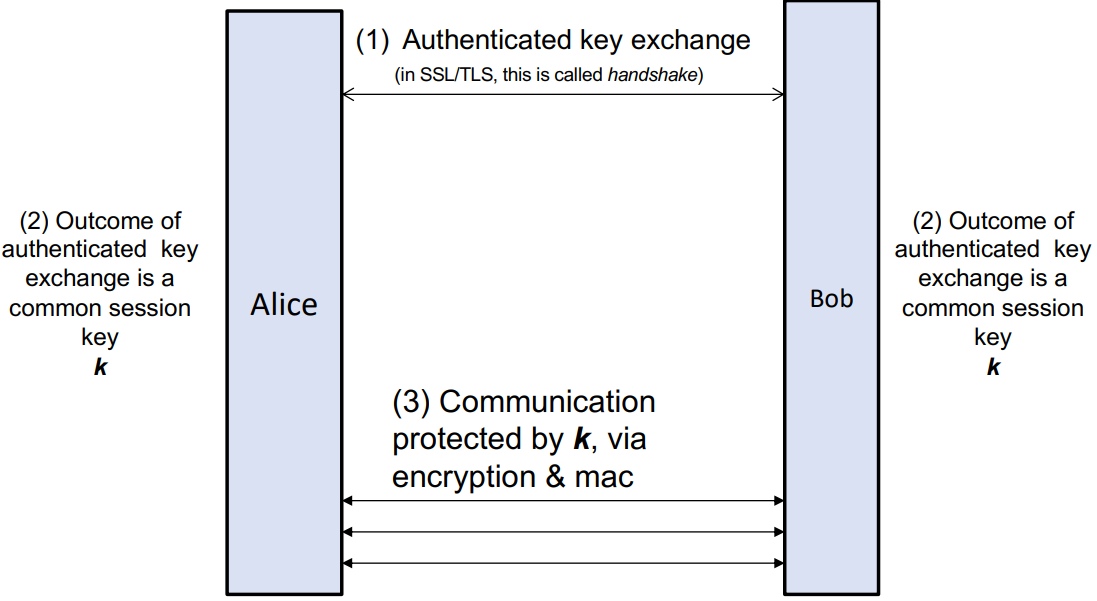
\includegraphics[width=8.5cm, height=4cm]{images/authkeyexchange.png} 

\begin{itemize}[noitemsep,wide=0pt, leftmargin=\dimexpr\labelwidth + 2\labelsep\relax]
    \item Authentication key-exchange: Outcome is a new shared secret \textbf{\textit{k}} known as \textbf{session key}.
    \item Subsequently, all communication will be protected (encrypted + mac) using \textbf{\textit{k}}.
\end{itemize}

\subsection*{Key-exchange || Sniff then Steal session key}
Alice and Bob want to establish a common key. Key can be used to protect subsequent communication.
The interaction could be eavesdropped by Eve, after sniffing, Eve wants to guess the established key.

\subsubsection{PKC-based Key-exchange}
\begin{enumerate}[noitemsep,wide=0pt, leftmargin=\dimexpr\labelwidth + 2\labelsep\relax]
    \item Alice generates a pair of private/public key
    \item Alice sends public key \textbf{k$_e$} to Bob
    \item Bob carries out the following:
    \begin{itemize}[noitemsep,wide=0pt, leftmargin=\dimexpr\labelwidth + 2\labelsep\relax]
        \item Randomly chooses secret \textbf{k}
        \item Encrypts \textbf{k} using \textbf{k$_e$}
        \item Sends the ciphertext \textbf{c} to Alice
    \end{itemize}
    \item Alice uses her private key \textbf{k$_d$} to decrypt and obtain \textbf{k}.
\end{enumerate}

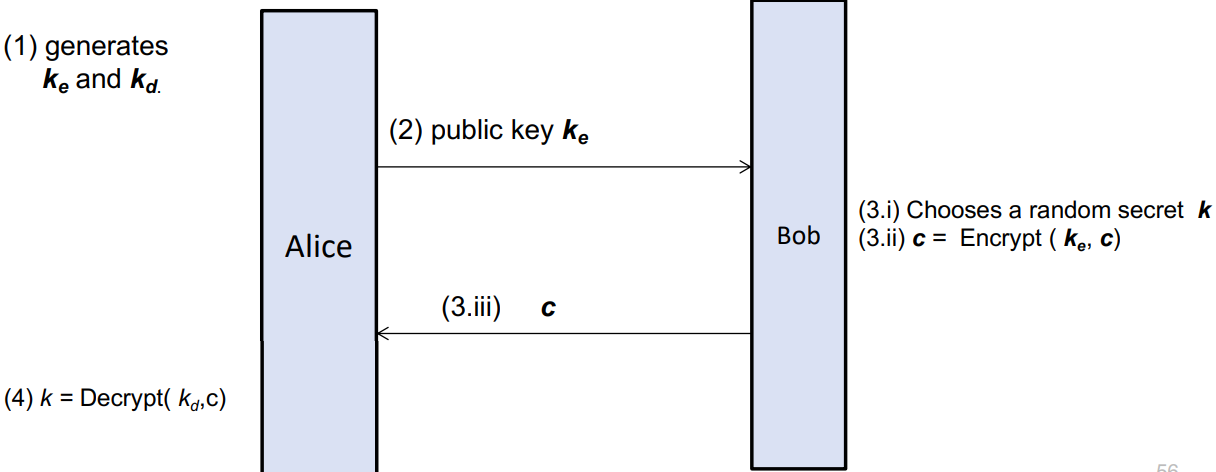
\includegraphics[width=8.5cm, height=3.5cm]{images/keyexchange.png} 

\begin{itemize}[noitemsep,wide=0pt, leftmargin=\dimexpr\labelwidth + 2\labelsep\relax]
    \item Attacker (Eve) can obtain public key \textbf{k$_e$} and the ciphertext \textbf{c}.
    \item By security of PKC, from the public and ciphertext, attacker cannot get any information of the plaintext, which is the key \textbf{k.}
\end{itemize}

\subsubsection{Diffie-Hellman Key-exchange}
We assume both Alice and Bob have agreed on two public parameters, a generator g and a
large (e.g. 1000 bits) prime p. Both g and p are not secret and known to the public

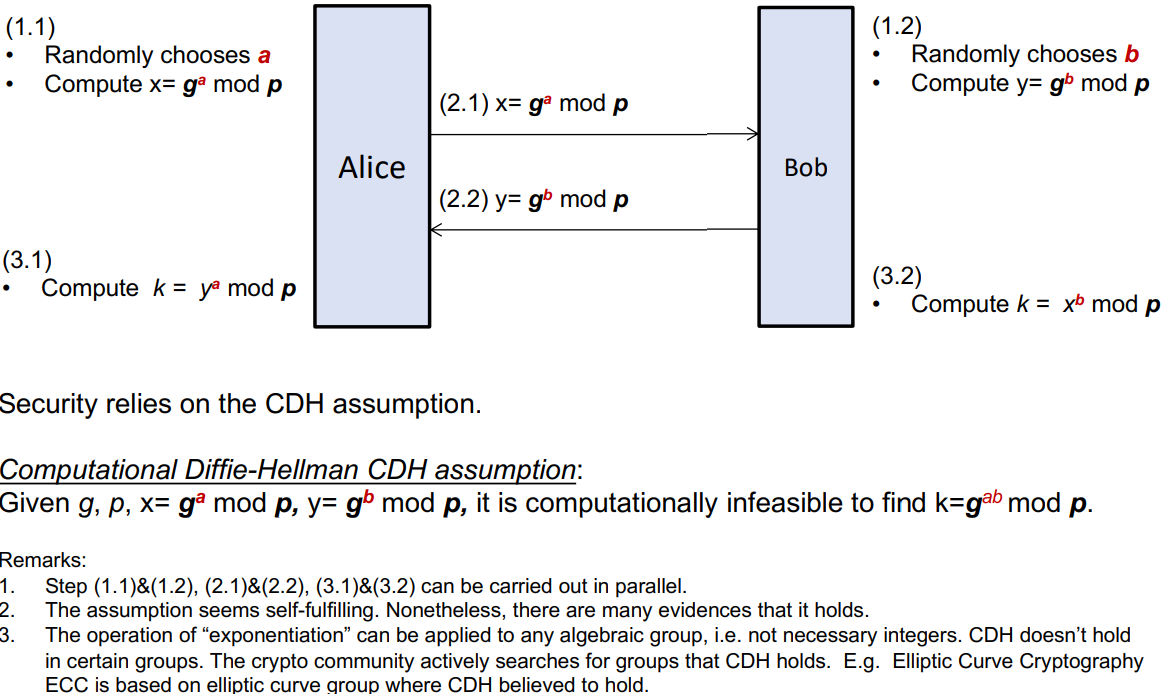
\includegraphics[width=8.6cm, height=6cm]{images/DiffieHellman.png} 

\subsection{Authenticated Key-exchange}
What if the adversary is malicious? Example, a man-in-the- middle?
In this case, Alice mistaken that Mallory is Bob. Communication from Alice
is encrypted using k$_A$. Mallory can decrypt using k$_A$ and re-encrypt using k$_B$.
Hence, Mallory can see and modify the message.

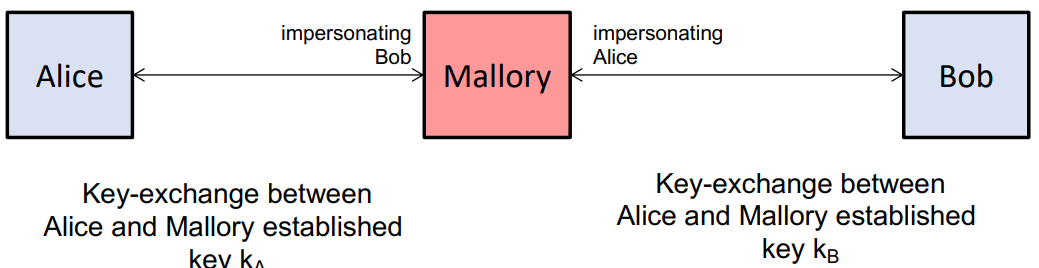
\includegraphics[width=8.6cm, height=2cm]{images/maninthemiddleauthkeyexchange.png} 
\begin{itemize}[noitemsep,wide=0pt, leftmargin=\dimexpr\labelwidth + 2\labelsep\relax]
    \item Key-exchange protocol assumes that the adversary can only \textit{sniff} but not malicious.
    \item Authenticated key-exchange can easily be obtained from existing key-exchange. (either PKC-based key-exchange
    or DH-based key-exchange). This can be done by signing all communication using private key.
\end{itemize}

\subsection{Station-to-Station protocol STS}
Authenticated key-exchange based on DH. We assume both Alice and Bob have agreed on two public parameters, a generator \textit{g} and a
large (e.g. 1000 bits) prime \textit{p}. Both \textit{g} and \textit{p} are not secret and known to the public.
Here, we consider unilateral authentication. Alice want to authenticate Bob.

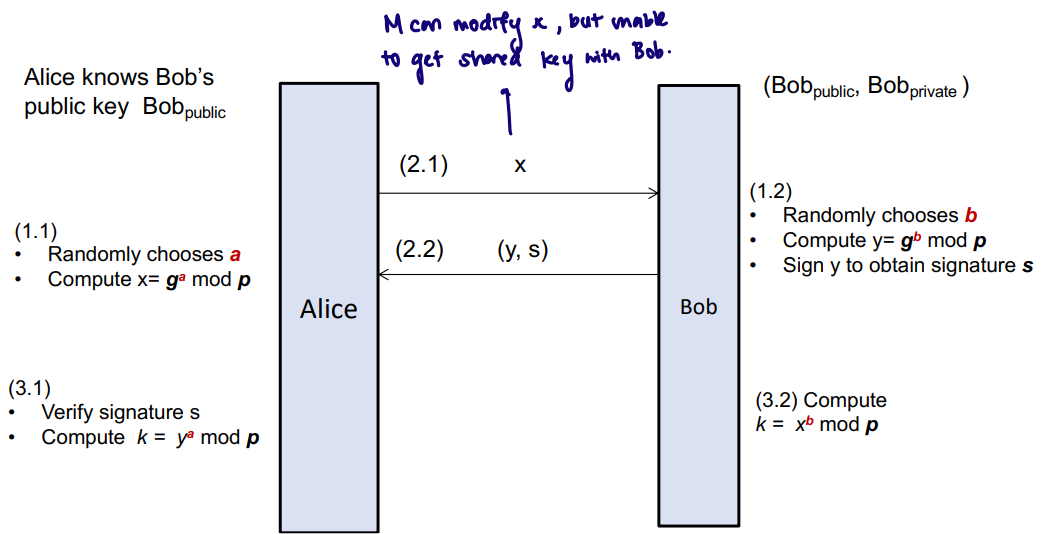
\includegraphics[width=8.6cm, height=4cm]{images/stsprotocol.png} 

\begin{itemize}[noitemsep,wide=0pt, leftmargin=\dimexpr\labelwidth + 2\labelsep\relax]
    \item (Asymmetric) Previous authenticated key-exchange protocols such as Station-to-station are
    based on public key. That is, an entity is considered authentic if it can convince the other
    that it know the private key of the associated public key.
    \item (Symmetric) There are also symmetric key version, i.e both entities share a symmetric key.
    An entity is authentic if it can prove to the other that it knows the key. 
    \item (Password) A special case of symmetric key is when the key is a password. Password
    usually has very low entropy, and thus potentially could be vulnerable to “offline”
    dictionary attack (see tutorial). There are secure protocols that, even if the entropy of
    password is low, it is still secure against offline dictionary attack. These are called “Password-Authenticated Key
    agreement” (PAKE). 
\end{itemize}

\subsubsection{Summary: Mutual Key-exchange}
\begin{itemize}[noitemsep,wide=0pt, leftmargin=\dimexpr\labelwidth + 2\labelsep\relax]
    \item Before the protocol:
    \begin{enumerate}[noitemsep,wide=0pt, leftmargin=\dimexpr\labelwidth + 2\labelsep\relax]
        \item Alice has a pair of public, private key (A$_{public}$ , A$_{private}$ ).
        \item Bob has a pair of public, private key (B$_{public}$ , B$_{private}$ ).
        \item Alice knows Bob public key and vice versa. These two sets of keys are known as
        the \textbf{\textit{Long-term key}} or \textbf{\textit{Master key}}.
    \end{enumerate}
    \item They carry out Authenticated key exchange protocol (e.g. STS). If an entity is not
    authentic, the other will halt. 
    \item After the protocol: Both A and B obtain a shared key \textbf{k}, known as the \textbf{\textit{Session key}}
    \item Security Requirement:
    \begin{itemize}[noitemsep,wide=0pt, leftmargin=\dimexpr\labelwidth + 2\labelsep\relax]
        \item (Authenticity) Alice is assured that she is communicating with an entity who
        knows B$_{private}$.
        \item (Authenticity) Bob is assured that he is communicating with an entity who knows
        Aprivate.
        \item (Confidentiality) Attacker unable to get the session key
    \end{itemize}
\end{itemize}

\subsection{Securing Communciation Channel || TLS}
Public channel facilitates communication, but not secure with presence of Mallory. We 
can use crypto primitive on the messages, so that it is as secure as a `private channel'.

Alice wants to visit a website \verb|Bob.com|. ALice using the free wifi in a cafe called Mallory.
How to secure the communication under the presence of malicious Mallory. In TLS/SSL:
\begin{enumerate}[noitemsep,wide=0pt, leftmargin=\dimexpr\labelwidth + 2\labelsep\relax]
    \item Using \textbf{long-term keys (i.e. Bob’s public and private key)}, carry out
    authenticated key-exchange (aka handshake in TLS). Outcomes are:
    \begin{itemize}[noitemsep,wide=0pt, leftmargin=\dimexpr\labelwidth + 2\labelsep\relax]
        \item Alice is convinced that she is interacting with Bob.
        \item Both Alice and Bob have a shared session key. Mallory unable to get the key.
    \end{itemize}
    \item Subsequent communication protected by the session key.
\end{enumerate}

\subsubsection*{TLS}
\begin{enumerate}[noitemsep,wide=0pt, leftmargin=\dimexpr\labelwidth + 2\labelsep\relax]
    \item Alice obtains \verb|Bob.com|’s public key. This is done by having Bob sending his certificate to Alice.
    \item Alice and Bob.com carry out \textbf{unilateral authenticated key exchange}
    protocol with Bob’s private/public key. After the protocol, both Bob and Alice obtain
    two shared keys \textbf{\textit{t}} , \textbf{\textit{k}} where \textbf{\textit{t}} is the secret key of the MAC, and \textbf{\textit{k}} is the secret key of
    the symmetric-key encryption, say AES. They are called the \textbf{\textit{session keys}}. From
    Alice’s point of view, the protocol is secure in the sense that, only an entity who
    knows Bob’s private key can complete the protocol. So, Alice is convinced that the
    entity who now holds \textbf{\textit{t}}, \textbf{\textit{k}} is Bob. Here, Bob doesn’t care about Alice’s authenticity.
    \item Subsequent interactions between Alice and Bob.com will be protected by
    \textbf{\textit{t}}, \textbf{\textit{k}} and a sequence number. Suppose m$_1$, m$_2$, m$_3$, … are the sequence of message
    exchanged, the actual data to be sent for m$_i$ is
    \begin{equation*}
        E_k ( i || m ) || mac_t ( E_k ( i || m) )
    \end{equation*} where \textit{i} is the sequence number. This is known as `encrypt-then-MAC'. There are other variants: `mac-then-encrypt' and `mac-and-encrypt'. Using
    the wrong variant might leak info. When in doubt, use “authenticated encryption” such as AES GCM mode. GCM is fairly
    new and was not established when TLS was designed.
\end{enumerate}

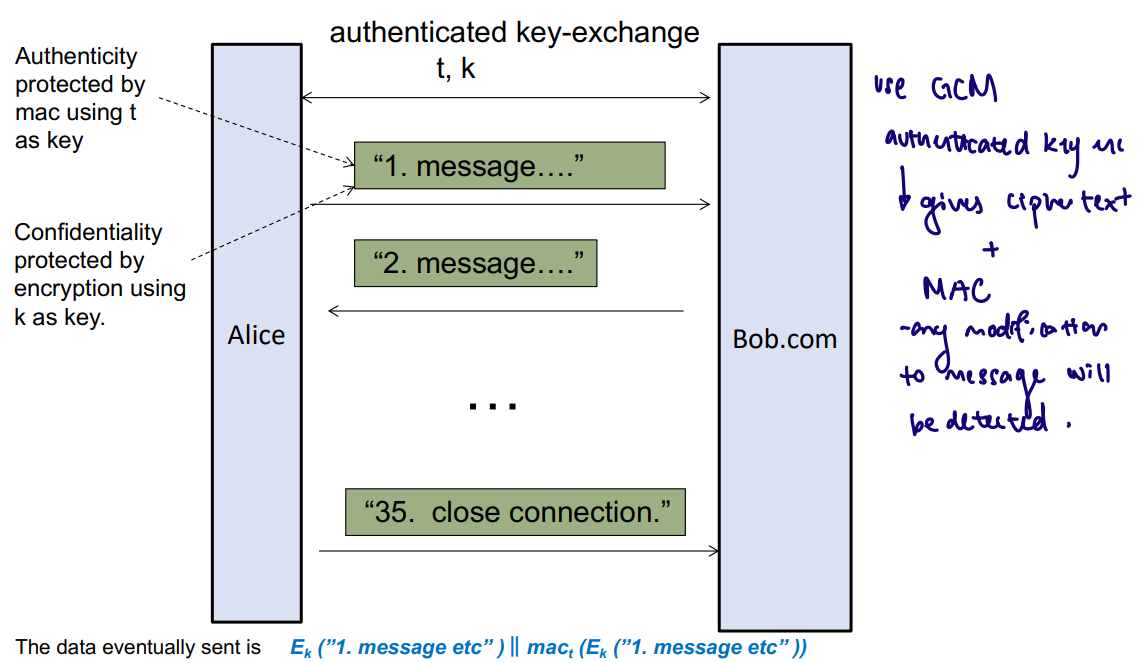
\includegraphics[width=8.6cm, height=4cm]{images/tls.png} 

SSL and Transport Layer Security (TLS) are protocols that secure communication using cryptographic means.
SSL is the predecessor of TLS and HTTPS is built on top of TLS.

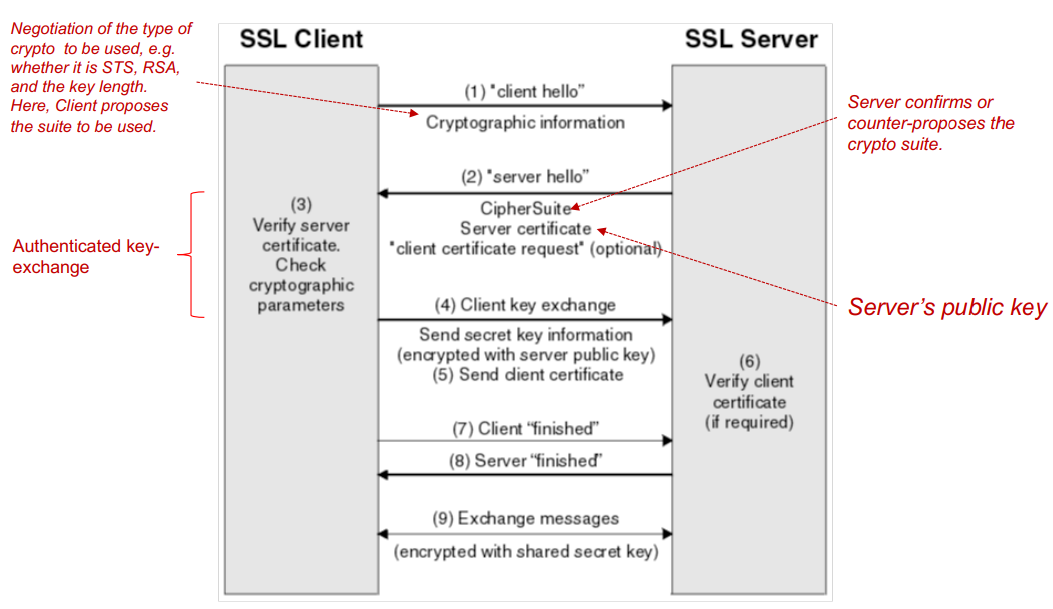
\includegraphics[width=8.6cm, height=4cm]{images/TLShandshake.png} 

\section*{\underline{Network Security}}
Computer Network establishes communicating connections between entities. To share networking resources 
and enhance robustness, instead of having dedicated lines between any 2 nodes, \textbf{packet switching} is deployed.
\begin{itemize}[noitemsep,wide=0pt, leftmargin=\dimexpr\labelwidth + 2\labelsep\relax]
    \item Messages route via multiple switches and routers $\rightarrow$ Messages are broken into packets/frames
    \item Network security focuses on effects on attackers among intermediate nodes. Attacker wants to steal, modify, disrupt CIA.
    \item \textbf{Routing}:
    \begin{enumerate}[noitemsep,wide=0pt, leftmargin=\dimexpr\labelwidth + 2\labelsep\relax]
        \item Route traffic to nowhere: Availability
        \item Know who is talking to who.
        \item Route traffic to attacker, become MITM. 
    \end{enumerate}
\end{itemize}

\subsubsection*{Multiple hops and netowrk layers}
To handle different types of intermediate nodes, network protocols are abstracted as layers. Conceptually, layer (N-1) provides a `virtual' channel
for entities in layer N. The \textit{peer entities} in the N layer communicate using the virtual channel in layer (N-1). In turn, 
layer N provide yet another virtual channel for layer N+1.
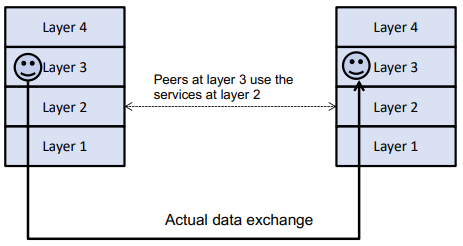
\includegraphics[width=8.6cm, height=3cm]{images/multiplehop.png} 
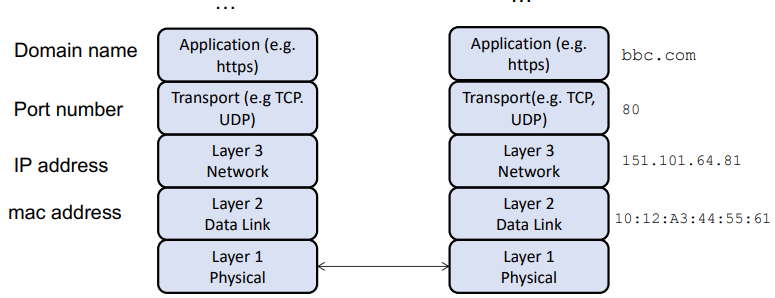
\includegraphics[width=8.6cm, height=3cm]{images/internetlayer.png} 

\begin{multicols*}{2}
    \begin{itemize}[noitemsep,wide=0pt, leftmargin=\dimexpr\labelwidth + 2\labelsep\relax]
        \item Domain name: \verb|bbc.com|
        \item Port Number: 60
        \item IP-address: 151.101.64.81
        \item MAC-address: 10:12:A3:44:55:61
    \end{itemize}
\end{multicols*}

\subsubsection*{Data units generated by layers}
\begin{itemize}[noitemsep,wide=0pt, leftmargin=\dimexpr\labelwidth + 2\labelsep\relax]
    \item Layer-N channel invoked to send message \textbf{n}, protocol in layer N might transform \textbf{m} into pieces of `payload'.
    Each payload has a header generated by protocol. Both header and payload forms a data unit in layer N to be sent by layer N-1.
    \item Layer N at receiver from a series of received data units, reconstruct back to \textbf{m}.
    \begin{itemize}[noitemsep,wide=0pt, leftmargin=\dimexpr\labelwidth + 2\labelsep\relax]
        \item Transport layer: datagram
        \item Network layer: packet
        \item Datalink layer: frame
    \end{itemize}
    \item Each header contains 2 pieces of information: (1) src address, sender's address (at layer N) and (2) dest address, receiver's address (at layer N)
\end{itemize}

\includegraphics*[width=8.5cm, height=4cm]{images/dataflowlayers.png}
\includegraphics*[width=8.5cm, height=4cm]{images/dataflowlayers2.png}

\subsubsection*{Intermediate nodes}
Data are routed through multiple hops. Intermediate nodes could be owned
by different third parties, e.g. Internet service provider (ISP), company’s
firewall. To facilitate routing, intermediate nodes see routing/header
information, and might also change them (e.g translate the address, add
“hop count”).

\subsection*{Man-In-The-Middle || MITM}
MITM sits between 2 communicating parties. Unless otherwise stated, the MITM can sniff, spoof,
modify, drop the data. Very often, when mentioning a MITM, it is clear from context what info the MITM has access to. 
\begin{itemize}[noitemsep,wide=0pt, leftmargin=\dimexpr\labelwidth + 2\labelsep\relax]
    \item \textbf{MITM sits in Layer 3}, MITM can see input (e.g. datagram, transport header) to Layer 3 and decide what the output of Layer 3 (packet, network header etc.) and know all internal info stored in Layer 3 (e.g. secret key).
    \item \textbf{MITM sits between Layer 2 and 3}, or just above layer 2, just below layer 3, we mean that the MITM can see and modify output of Layer 3, but do not have access to internal data in Layer 3.
\end{itemize}

\subsubsection*{Challenges in Network Security}
\begin{itemize}[noitemsep,wide=0pt, leftmargin=\dimexpr\labelwidth + 2\labelsep\relax]
    \item (Intermediate nodes and layers) There are many intermediate nodes, each handling routing-related information at a different layer. 
    \item (Security Requirements)
    \begin{itemize}[noitemsep,wide=0pt, leftmargin=\dimexpr\labelwidth + 2\labelsep\relax]
        \item \textbf{Availability} main concern in networking
        \item \textbf{Confidentiality and integrity of Routing}:
        \begin{itemize}[noitemsep,wide=0pt, leftmargin=\dimexpr\labelwidth + 2\labelsep\relax]
            \item Modifying routing process would break connections (availability) redirect traffic to adversary (confidentiality) ||could lead to side-channel leakages or implementation flaws if attacker can see ciphertext still.
            \item Leakage of routing information could reveal connectivity information like A talking to B $\rightarrow$ Anonymity and Privacy.
        \end{itemize}
        \item (Legacy and security tradeoff) Initial design of netowrking protocols did no consider intentional attacks. (e.g. DNS does not employ strong protoection mechanisms for performance sake.)
        \item (Management) There is a need to isolate and control data flow (firewall).
    \end{itemize}
\end{itemize}

\subsection*{TCP/IP and UDP/IP}
\subsubsection*{Transport Layer + IP}
\begin{itemize}[noitemsep,wide=0pt, leftmargin=\dimexpr\labelwidth + 2\labelsep\relax]
    \item Transport layer and IP layer often treated as a single layer: \textbf{ip-address} and \textbf{port number}.
    \item Each node in the network has a total of 65535 ports
    \item Communication channel between 2 nodes established by connecting 2 ports. e.g. between \verb|11.11.1.1:2| and \verb|55.55.5.5:65535|
\end{itemize}

\subsubsection*{UDP/IP}
\begin{itemize}[noitemsep,wide=0pt, leftmargin=\dimexpr\labelwidth + 2\labelsep\relax]
    \item \verb|DatagramSend(srcPort, destIp, destPort, message)|
    \item \verb|DatagramSend| library constructs an \textit{IP datagram} and then an \textit{IP packet} and passes to \textbf{Data Link layer}.
    \item There is a limit on the size of the array \verb|message| $\rightarrow$ 65,000 bytes.
    \item \verb|DatagramSend| does not return a result indicating whether the destination received the packer. There is a possibility that the packet is lost, arrived late or the recipient does not exist.
    \item UDP protocol is \textit{unreliable}, data might get lost of arrive in a different order.
\end{itemize}

\subsubsection*{TCP/IP: reliable communication}
\begin{itemize}[noitemsep,wide=0pt, leftmargin=\dimexpr\labelwidth + 2\labelsep\relax]
    \item Application make library calls in the following form:
    \begin{lstlisting}
P = open_connection(2, "33.43.100.2", 65535)
    send(P, out_message) // can have multiple 
    read(P, in_message)  // rounds of send/read
close_connection(P)
    \end{lstlisting}
    \item \verb|open_connection| carries out some form of handshake-protocol (TCP 3-way handshake) to make sure recipient is listening.
    \item \verb|send| constructs \textit{ip packets} of the following form and pass them to datalink layer. If message too long, form multiple ip packets.
    \item Protocol also has mechanism for \textit{re-sending}, \textit{re-ordering}, \textit{acknowledgement} to ensure destination did in fact receive the message.
\end{itemize}

\subsubsection*{Reliability does not imply Security}
\begin{itemize}[noitemsep,wide=0pt, leftmargin=\dimexpr\labelwidth + 2\labelsep\relax]
    \item TCP/IP reliable but not \underline{secure}. Intermediate nodes along communication route can still modify data in header or payload.
    \item Malicious intermediate node might act as MITM in IP layer.
    \begin{itemize}[noitemsep,wide=0pt, leftmargin=\dimexpr\labelwidth + 2\labelsep\relax]
        \item spoof IP packet to inform one node to close the connection
        \item reorder the packets
    \end{itemize}
\end{itemize}

\subsubsection*{Listening to a port / Closed port}
\begin{itemize}[noitemsep,wide=0pt, leftmargin=\dimexpr\labelwidth + 2\labelsep\relax]
    \item Behind certain ports, there are applications waiting to process data coming via the respective port. $\rightarrow$ node/process is listening to the port
    \item If port is not listening $\rightarrow$ closed port, data sent to closed port will be dropped.
\end{itemize}

\subsection*{Name Resolution and Attacks: DNS/ARP}
To use virtual connection in layer (N-1), need to know receiver name in layer (N-1) Method of finding
the corresponding name is called \textit{resolution} protocol.
\begin{itemize}[noitemsep,wide=0pt, leftmargin=\dimexpr\labelwidth + 2\labelsep\relax]
    \item \textbf{Domain Name System (DNS):} resolution of Domain name to IP address
    \item \textbf{Address Resolution Protocol (ARP):} resolution of IP address to MAC address
\end{itemize}

\subsubsection*{Domain Name System (DNS)}
Given a domain name e.g. www.comp.nus.edu.sg, ip address can be found by querying a remote DNS server.
The client who initiates the query is called the \textit{resolver}. If the address is found, we say
domain name is \textit{resolved}.

\includegraphics*[width=8.5cm, height=4.5cm]{images/dnsqueryandanswer.png}

\subsubsection*{DNS Spoofing: Attack scenario}
\textbf{WHEN NOT UNDER ATTACK}
\begin{itemize}[noitemsep,wide=0pt, leftmargin=\dimexpr\labelwidth + 2\labelsep\relax]
    \item Alice using cafe wifi to surf web and wants to visit and login to \underline{nus.edu.sg}.
    She types domain name into browser address bar.
    \item Browser makes query to DNS server to determine ip address (\verb|nslookup|)
    Browser obtains and connects to ip address.
\end{itemize}

\textbf{ATTACK}
\begin{itemize}[noitemsep,wide=0pt, leftmargin=\dimexpr\labelwidth + 2\labelsep\relax]
    \item Consider an attacker who is also in the cafe, since wifi no protected, attacker can
    \begin{itemize}[noitemsep,wide=0pt, leftmargin=\dimexpr\labelwidth + 2\labelsep\relax]
        \item sniff data from communication channel
        \item inject spoofed data into communication channel
    \end{itemize}
    \item Attacker cannot remove/modify data sent by Alice (sits below physical layer).
    \item Attacker owns a webserver at \verb|100.10.10.3| which is a spoofed NUS website. ATTACK:
    \begin{enumerate}[noitemsep,wide=0pt, leftmargin=\dimexpr\labelwidth + 2\labelsep\relax]
        \item Alice ask for address.
        \item Attacker sniffs and knows about it, quickly spoofs a reply with the same QID.
        \item DNS server also sends a reply, since attacker closer to Alice, their reply likely reaches Alice first.
        \item Alice takes first reply as answer and connects to spoof NUS website \verb|100.10.10.3|
    \end{enumerate}
    \includegraphics*[width=8.3cm, height=2.6cm]{images/dnspoisoning.png}
\end{itemize}

\includegraphics*[width=8.3cm, height=3.5cm]{images/dnsspoofing.png}
\begin{itemize}[noitemsep,wide=0pt, leftmargin=\dimexpr\labelwidth + 2\labelsep\relax]
    \item DNS important component as it resolves domain name, can be a \underline{single-point of failure} of network.
    \item DDOS attacks on web service, instead of directly attacking server, could conduct DOS to DNS server instead. $\rightarrow$
    When DNS server downed, web service no longer reachable.
\end{itemize}

\subsubsection*{Poisoning Attack on ARP Table}
A switch connects a few nodes. There is one node N$_0$ that acts as a gateway, which is a virtual node in the switch device that connects to the Internet.
\begin{itemize}[noitemsep,wide=0pt, leftmargin=\dimexpr\labelwidth + 2\labelsep\relax]
    \item Switch is similar to telephone switchboard, it connects 2 ports.
    \item Switch does not understand ip-addresses and does not store ip-addresses (router), it conencts ports based on MAC-addresses.
    \item Switch keeps a table that maps port to MAC-addresses.
    \item Resolution of ip-address to MAC-address is done by nodes, each node also has a switch table.
    \item Nodes update each other using protocols on information on ip/MAC-addresses
\end{itemize} 

\textbf{ARP Poisoning} is an attack that modifies (poison) the tables so as to gain MITM access

\subsubsection*{ARP Poisoning attack}
Under normal circumstances,, these are carried out when N$_2$ sends a packet to 10.0.1.4.
\begin{enumerate}[noitemsep,wide=0pt, leftmargin=\dimexpr\labelwidth + 2\labelsep\relax]
    \item N$_2$ looks up the table \textbf{T2}, resolved to \underline{fa:16:3e:ed:05:e4}.
    \item N$_2$ sends the frame to switch, with destination \underline{fa:16:3e:ed:05:e4}.
    \item Switch looks up table \textbf{T0}, redirect frame to port 3.
\end{enumerate}

Suppose N$_1$ wants to be MITM between 10.0.3.5 and 10.0.1.4
\begin{enumerate}[noitemsep,wide=0pt, leftmargin=\dimexpr\labelwidth + 2\labelsep\relax]
    \item N$_1$ informs N$_2$ that MAC address of 10.0.1.4 is \underline{\textbf{fa:16:3e:d5:e0:14}}.
    \item N$_1$ informs N$_3$ that MAC address of 10.0.3.5 is \underline{\textbf{fa:16:3e:d5:e0:14}}.
\end{enumerate}

After tables are \textbf{poisoned}, all frames will be sent to N$_1$, which can relay the frames,
modify the frames before relaying. N$_1$ becomes MITM in layer 2.

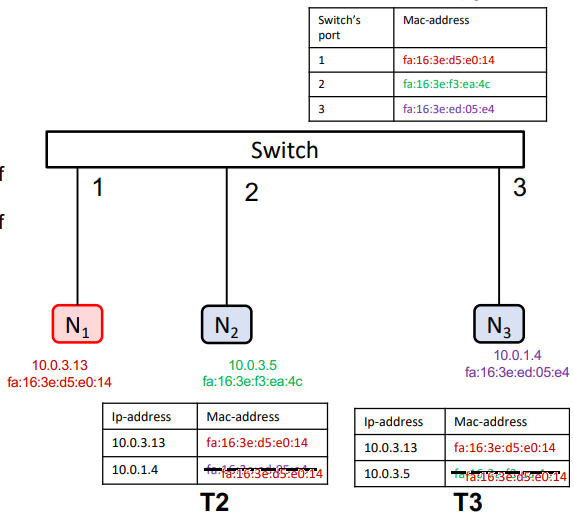
\includegraphics[width=6cm, height=4cm]{images/MITMarp.png}

\subsection*{Denial of Service Attack}
DOS is an attack on availability. 
\begin{itemize}[noitemsep,wide=0pt, leftmargin=\dimexpr\labelwidth + 2\labelsep\relax]
    \item \textbf{Availability:} The property of being accessible and usable upon demand by an authorized entity.
    \item \textbf{Denial of service (DOS):} The prevention of authorized access to resources or the delaying of time-critical operations.
    \item Many successful DOS attacks simply flood the victims with overwhelming requests/data.
\end{itemize}

\subsubsection*{Example of DOS attack}
E.g. MyDoom worm which targeted SCO's website. Attacks start on Feb 12, 2004, sending a large number of DNS requests to the DNS server.
For DOS to be effective, large number of attackers required. When DOS is carried out by large number of attackers,
called DDOS: \textbf{Distributed Denial of Service}.

\subsubsection*{Reflection Attack}
Reflection attack is a type of DOS in which the attackers send requests to
intermediate nodes, which in turn send overwhelming traffic to the
victim. Indirect, and thus more difficult to trace.

\subsubsection*{Amplification Attack}
Refection attack mechanism can be measured by its amplification factor,
which is the size of traffic the victim received over the size of traffic sent
by the attacker. A single request could trigger multiple responses from the intermediate
nodes. Reflection attack aka amplification attack.

\subsubsection*{Example of Reflection attacks: ICMP/Smurf Flood}
This attacker is no longer effective, as routers are configured to not broadcast by default.
\begin{enumerate}[noitemsep,wide=0pt, leftmargin=\dimexpr\labelwidth + 2\labelsep\relax]
    \item Attacker sends request \verb|ICMP PING| to router, instructing router to broadcast request. Source ip-address of request is spoofed with victim ip address.
    \item Router broadcast this request.
    \item Each entity who has received this request, replies to it by sending an `echo reply' to the source which is the victim.
    \item Victim's network overwhlemed with the echo reply.
\end{enumerate}

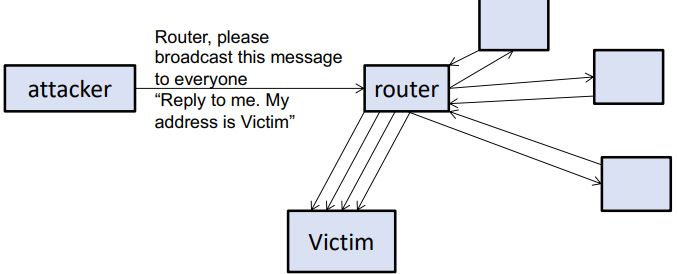
\includegraphics[width=8.5cm, height=3cm]{images/broadcastattack.png}

\subsubsection*{Example of Reflection attacks: DNS reflection attack}
During a DNS amplification attack, the perpetrator sends out a DNS query with a
forged IP address (the victim’s) to an open DNS resolver, prompting it to reply back to
that address with a DNS response. With numerous fake queries being sent out, and
with several DNS resolvers replying back simultaneously, the victim’s network can
easily be overwhelmed by the sheer number of DNS responses. (e.g. Github using Memcache on 5 Mar 2018.)

\subsection*{Botnet}
\begin{itemize}[noitemsep,wide=0pt, leftmargin=\dimexpr\labelwidth + 2\labelsep\relax]
    \item \textbf{Bot}: aka \textit{zombie} is a ccompromised machine
    \item \textbf{Botnet}: aka \textit{zombie army} is a large collection of
    connected bots, communicating via covert channels.
    \item A botnet has a command-and-control mechanism, and thus can be control by an individual to carry out DDOS.
    \item Possible usages of a botnet:
    \begin{itemize}[noitemsep,wide=0pt, leftmargin=\dimexpr\labelwidth + 2\labelsep\relax]
    \item DDoS flooding, vulnerability scanning, anonymizing
    \item HTTP proxy, email address harvesting, cipher breaking
    \end{itemize}
\end{itemize}

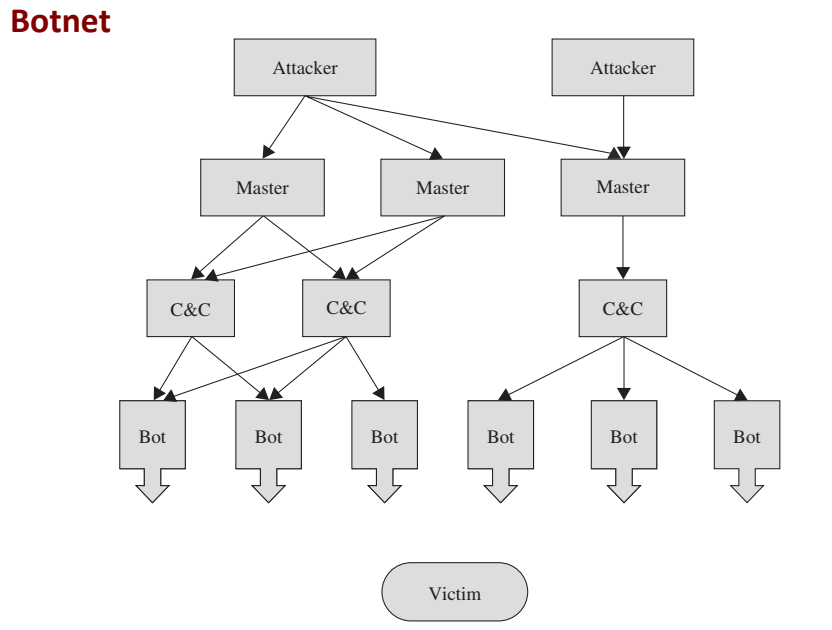
\includegraphics[width=8.5cm, height=5cm]{images/botnet.png}
\begin{itemize}[noitemsep,wide=0pt, leftmargin=\dimexpr\labelwidth + 2\labelsep\relax]
    \item there is a new trend of using `non-PC' such as IoT devices as bots in launching DDOS.
\end{itemize}

\subsection*{Useful tools}
\subsubsection*{Wireshark || Packet Analyzer}
\begin{itemize}[noitemsep,wide=0pt, leftmargin=\dimexpr\labelwidth + 2\labelsep\relax]
    \item Wireshark listens to “interactions” between the OS
    and the network card driver. (In other words, it is
    a MITM between OS and network card).
    \item Hence, header added by the network card, or
    modification made by the network card, may not
    be captured by Wireshark. This depends on the
    OS and the hardware. (usually Wireshark operates in layer 2)
\end{itemize}

\subsubsection*{Nmap || Port Scanning}
\begin{itemize}[noitemsep,wide=0pt, leftmargin=\dimexpr\labelwidth + 2\labelsep\relax]
    \item Multiple processes running in a server. When the server receives a packet, base on the port number, it will decide which process
    handle that packet. So, by saying that a process/service is \textbf{“listening”} to a particular \textbf{port}, we mean that the
    process is running and ready to handle arriving packets with that particular port number.
    \item When a port is \textbf{“open”}, there exist such a process running in the server. When a port is \textbf{“closed”}, no process is
    listening to that port.
    \item If a port is \textbf{“closed”}, attacker is unable to feed malicious data to that port.
\end{itemize}

\begin{itemize}[noitemsep,wide=0pt, leftmargin=\dimexpr\labelwidth + 2\labelsep\relax]
    \item \textbf{Port scanning:} process of determining which ports are open in a network
    \item \textbf{Port scanner:} tool used for port scanning. \textbf{Port scanning} is a useful tool for attacker, and network administrator to scan for vulnerabilites.
\end{itemize}

\subsection*{Protection || Secure communication channel}
Very often, when referring to a security protocol, we indicate the “layer” the
protocol targets to protect. When analyzing an attack, it is also insightful to figure out at what layer the
attacker resides. \\ 

A security protocol that protects layer k, would protect information in that
layer and above. Hence, if an attacker resides at layer 1, and there is a security protocol
that protect layer 3, then information generated in layer 3 and above will
be protected, but information generated in layer 2 would not be protected
by the security protocol 

\subsubsection*{SSL/TLS}
SSL/TLS sit on top of transport layer. When an application wants to send data to the other end point, it first
passes the data and the ip address to SSL/TLS. SSL/TLS first `protects' the data using encryption (confidentiality) and 
MAC (authenticity) and then instructs the transport layer to send the protected data. \newline

Suppose Alice uses LumiNUS to upload a report \verb|a.pdf| to LumiNUS server, LumiNUS uses HTTPS (HTTP on top of TLS.) \\

Alice’s machine carries the following:
\begin{enumerate}[noitemsep,wide=0pt, leftmargin=\dimexpr\labelwidth + 2\labelsep\relax]
    \item The LumiNUS application passes the file \verb|a.pdf| to https, and then to TLS.
    \item TLS protects the data by encryption and mac.
    \item TLS passes the protected data to the transport layer.
\end{enumerate}

LumiNUS’s server carries out the following:
\begin{enumerate}[noitemsep,wide=0pt, leftmargin=\dimexpr\labelwidth + 2\labelsep\relax]
    \item The transport layer passes the protected data to TLS.
    \item TLS decrypt the data and verify the mac for integrity.
    \item TLS passes the decrypted data to LumiNUS’s application. 
\end{enumerate}

\subsubsection*{Scenario 1 || Attacker @ Physical Layer}
Attacker at physical layer who can sniff/spoof message at that layer. Alice uploading her report in cafe
using free wifi (without WPA protectection). $\rightarrow$ anyone in the cafe has access to the physical layer and thus
can sniff and spoof messages in that layer.

\begin{itemize}[noitemsep,wide=0pt, leftmargin=\dimexpr\labelwidth + 2\labelsep\relax]
    \item Attacker cannot learn Alice's report, as data is encrypted by TLS $\rightarrow$ attacker only sees encrypted report.
    \item Attacker can learn the Alice is visiting LumiNUS website, since only those above TSL/SSL layer encrypted. Network layer is not encrypted,
    meaning attacker can still see the ip.
\end{itemize}
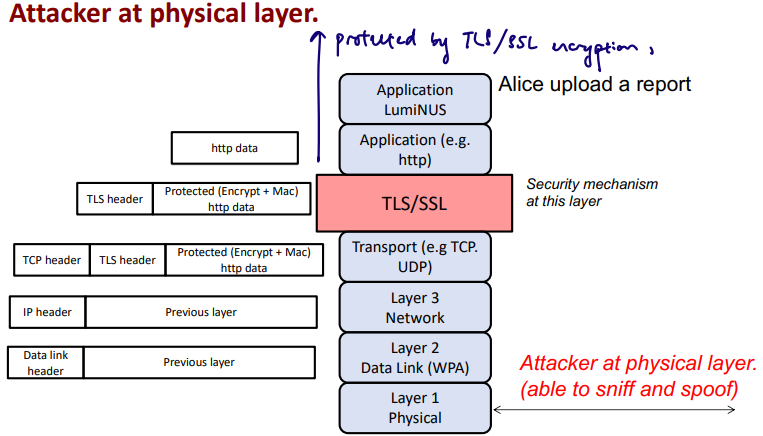
\includegraphics[width=8.5cm, height=5cm]{images/scenario1attack.png}

\subsubsection*{Scenario 2 || Adversary @ Application Layer}
Adversary in application layer, e.g. malicious javascript injected into LumiNUS, executed on Alice's browser.
\begin{itemize}[noitemsep,wide=0pt, leftmargin=\dimexpr\labelwidth + 2\labelsep\relax]
    \item Attacker can learn Alice's report AND can learn Alice's MAC-address.
\end{itemize}
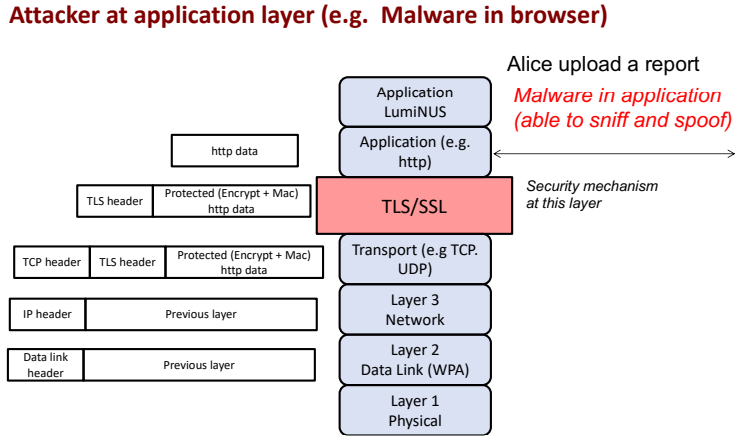
\includegraphics[width=8.5cm, height=5cm]{images/scenario2attack.png}

\subsection*{WPA2}
\textit{Wifi Protected Access II (WPA2)} is a popular protocol employed in home Wifi access point.
WPA2 provides protection at layer 2 (Link) and layer 1 (Physical). Not all information in layer 2 is protected.

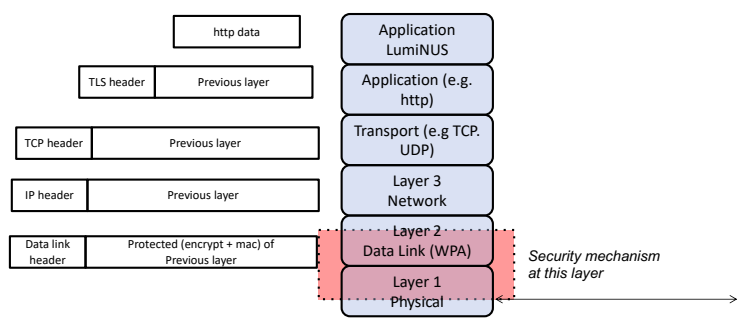
\includegraphics[width=8.5cm, height=3cm]{images/wpa2protection.png}

\subsubsection*{Scenario 3 || Attacker @ physical layer}
Attacker at physical layer and is able to sniff and spoof.
\begin{itemize}[noitemsep,wide=0pt, leftmargin=\dimexpr\labelwidth + 2\labelsep\relax]
    \item Attacker cannot learn Alice's report and cannot learn the fact that Alice is visiting LumiNUS website, since above Layer 2 is encrypted.
    \item Attacker is able to determine MAC-address of Alice.
\end{itemize}

\subsection*{IPSec}
IPSec provides “integrity/authenticity” protection of ip-address, but not
confidentiality. Hence, attackers are unable to “spoof” the source ip-source, but
can learn the source and destination ip-address of the sniffed packets.

\begin{itemize}[noitemsep,wide=0pt, leftmargin=\dimexpr\labelwidth + 2\labelsep\relax]
    \item IPSec needs to modify the OS, and is a mechanism whose goal is to protect the IP Layer.
    \item Internet Protocol Security (IPsec) is a protocol suite for securing Internet Protocol (IP)
    communications by authenticating and encrypting each IP packet of a communication
    session. IPsec includes protocols for establishing mutual authentication between agents at
    the beginning of the session and negotiation of cryptographic keys to be used during the
    session. IPsec can be used in protecting data flows between a pair of hosts (host-to-host),
    between a pair of security gateways (network-to-network), or between a security gateway
    and a host (network-to-host).
    \item Internet Protocol security (IPsec) uses cryptographic security services to protect
    communications over Internet Protocol (IP) networks. IPsec supports network-level peer
    authentication, data origin authentication, data integrity, data confidentiality (encryption),
    and replay protection.
    \item IPsec is an end-to-end security scheme operating in the Internet Layer of the Internet
    Protocol Suite, while some other Internet security systems in widespread use, such as
    Transport Layer Security (TLS) and Secure Shell (SSH), operate in the upper layers at
    Application layer. Hence, only IPsec protects any application traffic over an IP network.
    Applications can be automatically secured by IPsec at the IP layer.”
\end{itemize}

\subsection*{Firewall}
Some nodes contain more sensitive information than others. Some nodes are more \underline{secure}, available patches might take some time to 
patch all systems and need these secure nodes to be prioritized. Certain protocols do not have protection / light-weight protection mechanisms.
As such Firewall, Intrusion detection system (IDS) used to control access to the network.

\subsubsection*{Principle of least privilege and compartmentalization}
\begin{itemize}[noitemsep,wide=0pt, leftmargin=\dimexpr\labelwidth + 2\labelsep\relax]
    \item The principle of least privilege (PoLP, also known as the principle of
    minimal privilege or the principle of least authority) requires that in a
    particular abstraction layer of a computing environment, every module
    (such as a process, a user, or a program, depending on the subject) must be
    able to access only the information and resources that are necessary for its
    legitimate purpose.
    \item \textbf{Compartmentalization:} Generally, it refer to the notion of confining
    information within compartments. 
\end{itemize}

\begin{itemize}[noitemsep,wide=0pt, leftmargin=\dimexpr\labelwidth + 2\labelsep\relax]
    \item Firewall controls what traffic is allowed to enter the network \textbf{(ingress filtering)} or leave the network \textbf{(egress filtering)}.
    \item Firewalls are devices or programs that control the flow of network traffic between networks or hosts that employe differing security polices.
    \item \textbf{DMZ:} Demilitarized zone. A sub-network that exposes the organization’s external service to the (untrusted) Internet.
\end{itemize}

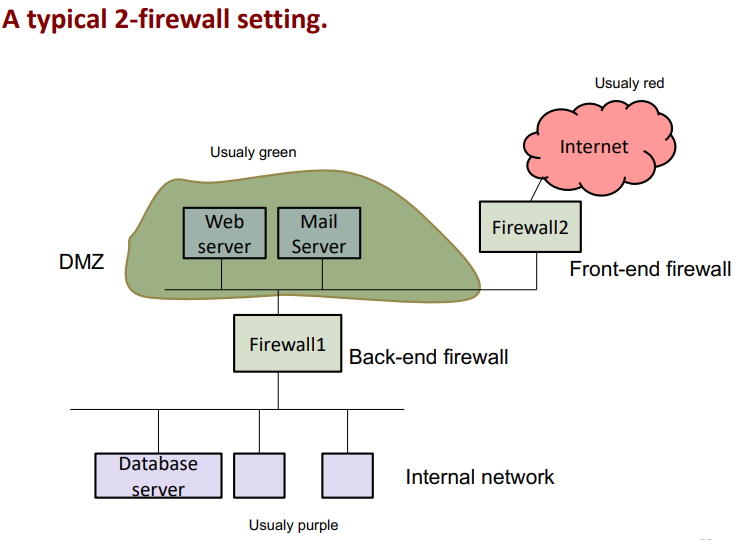
\includegraphics[width=8.5cm, height=5cm]{images/2-firewall.png}

Firewall's controls are achieved by \underline{packet filtering}. Filtering may occur in router, gateway/bridge or host.
Packet Filtering inspects every single packet, typically only the TCP/IP packet's header information (Network and Transport layer).
If payload is inspected, we call it a \textbf{\textit{deep packet inspection (DPI)}}. Actions taken after inspection:
\begin{multicols*}{2}
    \noindent
    \begin{itemize}[noitemsep,wide=0pt, leftmargin=\dimexpr\labelwidth + 2\labelsep\relax]
        \item Allow packet to pass
        \item Drop packet
        \item Reject the packet (drop + inform sender)
        \item Log info
        \item Notify system admin
        \item Modify packet (advanced devices)
    \end{itemize}
\end{multicols*}

\subsubsection*{Firewall Rules}
A firewall enforces a set of rules provided by the network administrator.
\begin{itemize}[noitemsep,wide=0pt, leftmargin=\dimexpr\labelwidth + 2\labelsep\relax]
    \item Drop packets with “source ip-address” not within the
    organization’s network. (To stop attacks originated within
    the network).
    \item \textbf{Whitelist:} Drop all packets except those specified in the white-list. (e.g. drop all
    except http, email protocol, and DNS)
    \item \textbf{Blacklist:} Accept all packets except those specified in the black-list. (e.g. allow
    https except ip-address in the blacklist).
\end{itemize}

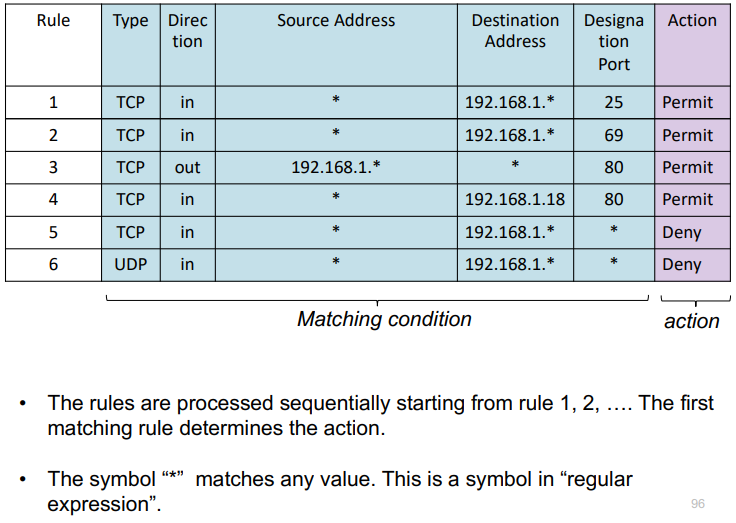
\includegraphics[width=8.5cm, height=5cm]{images/firewallrules.png}

\subsubsection*{Types of Firewalls}
NIST's document groups firewalls into 3 types
\begin{enumerate}[noitemsep,wide=0pt, leftmargin=\dimexpr\labelwidth + 2\labelsep\relax]
    \item Packet filters (inspect packet header)
    \item Stateful Inspection (Deep packet inspection) || e.g. count number of connections made in past hour
    \item Proxy (Modify packets)
\end{enumerate}

\subsection*{Intrusion Detection System}
An IDS system consists of a set of “sensors” who gather data. Sensors could
be in the host, or network router. The data are analyzed for intrusion.
Three types of IDS:
\begin{itemize}[noitemsep,wide=0pt, leftmargin=\dimexpr\labelwidth + 2\labelsep\relax]
    \item \textbf{Attack signature Detection:} The attack has specific, well-defined signature. For e.g. using certain port
    number, certain source ip address.
    \item \textbf{Anomaly Detection:} The IDS attempt to detect abnormal pattern. For e.g. a sudden surge of
    packets with certain port number.
    \item \textbf{Behavior-based IDS:} Can be viewed as a type of anomaly detection that focuses on human
    behavior. For e.g. The system might keep the profile of each user. It then
    tries to detect any user who deviates from the profile (e.g. start to download
    large files).
\end{itemize}

\subsection*{Management}
\begin{itemize}[noitemsep,wide=0pt, leftmargin=\dimexpr\labelwidth + 2\labelsep\relax]
    \item Management needed in order to monitor + adjust network characteristics
    \item \textbf{Security Operations Center (SOC):} a centralized unit in an organization that monitors the IT systems and
    deals with security issues
    \item \textbf{Security Information and Event Management (SIEM)}: Pronounced as “SIM”. Approaches and tools for SOC.
    Popular systems: Splunk ( https://www.splunk.com/ ), ELK Stack – Elasticsearch and Kibana (open sourced)
\end{itemize}

\section*{\underline{Access Control}}
We want to restrict \textbf{operations} on \textbf{objects} by \textbf{subjects}. Access control provides security perimeter which in
turn facilitates segregation of accesses. Such segregation confines and localize damage caused by attacks.

\subsection*{Security Perimeter}
Access controls setup perimiters/boundaries. With boundary, malicious activities outside of boundary would not affect resources within perimiter, and stays within boundary. Designed by the following principles:
\begin{itemize}[noitemsep,wide=0pt, leftmargin=\dimexpr\labelwidth + 2\labelsep\relax]
    \item \textbf{Principle of Least privilege: }A camera apps shouldn’t need to have access to the contact list to function. So, it is better not to grant the
    camera apps access to the contact list. With that, in case the camera app is malicious, confidentiality of the
    contact still preserved. 
    \item \textbf{Compartmentalization:} A school website hosts two services: (1) course’s fee payment and (2) exam result. With the perimeter between
    them, the exam result system would remain intact even if an SQL injection attack has been successfully carried
    out on the fee payment system. 
    \item \textbf{Compartmentalization:} Colonial Pipeline’s ransomware attack compromised the IT’s system that handle client’s database. If proper
    perimeter being setup between the IT and OT (Operation Technology) system, the failure of the client’s
    database system should not affect OT system that manages the fuel pipeline.
    \item \textbf{Defence in depth:} A company deploys a firewall separating their server from DMZ. In addition, activities of server is logged and
    regularly inspected. So, even if attacker able to sneak in, their activities could be discovered by the monitoring
    team. 
    \item \textbf{Segregation of duties:} A company keeps a backup copy of the “production” copy. The company implements a policy: a single person
    must not have access to both the production copy and the backup copy. Assigning different components to
    different person is aka Segregation of Duties. The goal is to eliminate single-point-of-failure. With that, a single
    rogue system admin (insider) is unable to corrupt all the data. 
\end{itemize}

\subsection*{Terminologies}
A \textit{principal} (or subject) wants to access an object with some operation. The
\textit{reference monitor} either grants or denies the access. Principal $\rightarrow$ Do operation $\rightarrow$ Reference Monitor $\rightarrow$ Object
\begin{itemize}[noitemsep,wide=0pt, leftmargin=\dimexpr\labelwidth + 2\labelsep\relax]
    \item \textbf{Principals vs Subjects:} Principals are human users, Subjects are entities in system operating on behalf of principals.
    \item Accesses to objects can be:
    \begin{itemize}[noitemsep,wide=0pt, leftmargin=\dimexpr\labelwidth + 2\labelsep\relax]
        \item \textbf{Observe:} \textit{read the file}
        \item \textbf{Alter:} Writing/Deleting or changing file properties
        \item \textbf{Action:} Executing a program
    \end{itemize}
    \item \textbf{Owner:} Who decides access rights to object?
    \begin{itemize}[noitemsep,wide=0pt, leftmargin=\dimexpr\labelwidth + 2\labelsep\relax]
        \item \textbf{Discretionary AC:} Owner object decides the rights.
        \item \textbf{Mandatory AC:} System-wide policy decides, strict rules everyone follows.
    \end{itemize}
\end{itemize}

\subsection*{Access Control Matrix}
Specify access rights of a particular principal to particular object.
\verb|r:read, w:write, x:execute, s: execute as owner, o: owner|

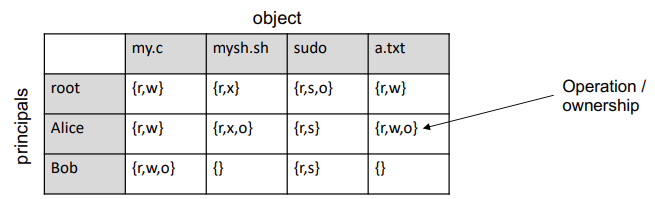
\includegraphics[width=8.5cm, height=2.4cm]{images/acm.png}

\subsubsection*{Access Control List}
ACL stores access rights to an object as a list.
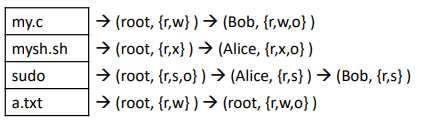
\includegraphics[width=5.5cm, height=1.5cm]{images/acl.png}

\subsubsection*{Capabilities}
A subject is given a list of capabilities, where each capability is the access rights to an object.
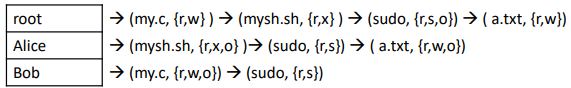
\includegraphics[width=8.5cm, height=1.5cm]{images/capability.png}

For ACL, it is difficult to obtain the list of objects a particular subject has access to.
Conversely, for capabilities, it is difficult to get the list of subjects who have access to
a particular object.

\subsection*{Intermediate Control}
Not practical for an owner to specific each single entries in the access control
matrix. “Group” the subjects/objects and define the access rights on the group. \\ 

In Unix file permission, subjects are divided into groups. Unix file permission uses ACL.
For each object, the owner specific the rights for \verb|owner|, \verb|group|, \verb|world| (everyone).

\subsubsection*{Role-based access control}
Grouping can be determined by the role of the subject. Role associates with a collection of procedures, 
in order to carry them out, access rights to certain objects are required.

\subsubsection*{Privelleges}
We sometime use the term privilege to describe the access right. Privilege can also be viewed as an intermediate
control. It can be represented by a number, e.g. 1,2,3. if a subject can access an object, another subject with
higher privilege can also access the object. (Can be viewed as a ladder, p2 subset of what p3 can access.)

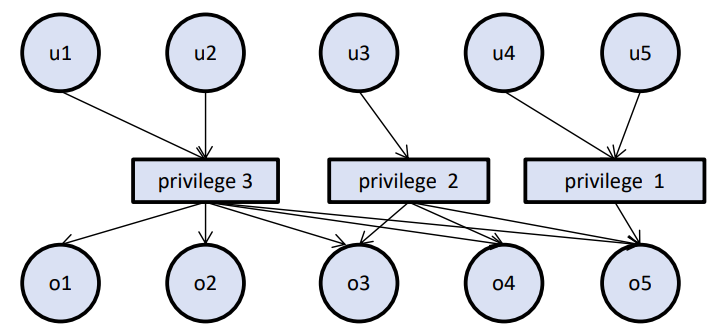
\includegraphics[width=8.5cm, height=3cm]{images/privilege.png}


\subsubsection*{Protection Rings}
In OS, “privilege” is often called protection rings. They are the same but
with different name. Here, each object (data) and subject (process) is
assigned a number. Whether a subject can access an object is determined
by their respective assigned number. Object with smaller number are more
important. If a process is assigned a number i, we say that the process runs
in ring i. We call processes with lower ring number as having “higher
privilege”. A subject cannot access (both read/write) an object with smaller ring
number. 

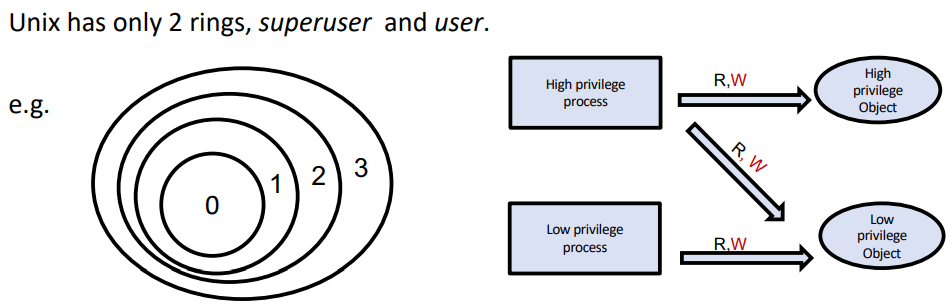
\includegraphics[width=8.5cm, height=3cm]{images/rings.png}

\subsubsection*{Bell-LaPadula Model || data confidentiality}
The following restrictions are imposed by the model:
\begin{itemize}[noitemsep,wide=0pt, leftmargin=\dimexpr\labelwidth + 2\labelsep\relax]
    \item \textbf{No read up:} A subject does not have read access to object in higher level. This prevent a lower level from
    getting info in the higher level.
    \item \textbf{No write down:} A subject does not have append-right to object in lower level. This prevents a malicious
    insider from passing information to lower levels. (e.g. a clerk working in the highly classified department is
    forbidden to gossip with other staff).
    \item For “Confidentiality”. (A subject can append to objects at higher security level. Is it possible that, by appending to an object, one could distort its original content? Yes.
    See e.g. in renegotiation attack.)
\end{itemize} 

\subsubsection*{Biba Mode || process integrity}
The following restrictions are imposed by the model:
\begin{itemize}[noitemsep,wide=0pt, leftmargin=\dimexpr\labelwidth + 2\labelsep\relax]
    \item \textbf{No write up:} A subject does not has “write” access to objects in higher level. This prevent a malicious subject
    from poisoning upper level data, and thus ensure that a process will not get compromised by lower level
    subjects.
    \item \textbf{No read down:} A subject does not has read access to objects lower level. This prevents a subject from reading
    data poisoned by lower level subjects. 
    \item For “Integrity”. If a model imposes both Biba and Bell-LaPadula, subjects can only read/write to objects in the same level (not
    practical).
\end{itemize} 
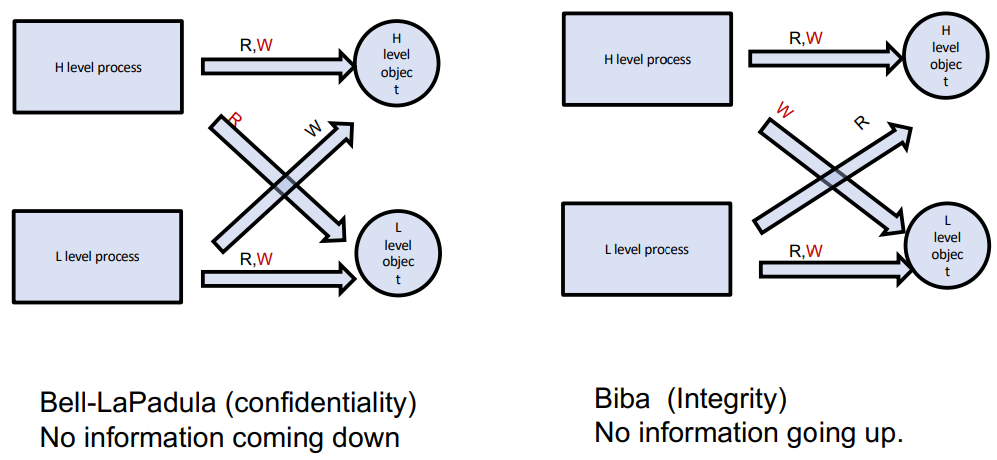
\includegraphics[width=8.5cm, height=3.5cm]{images/bellbiba.png}

\subsection*{Unix File System}
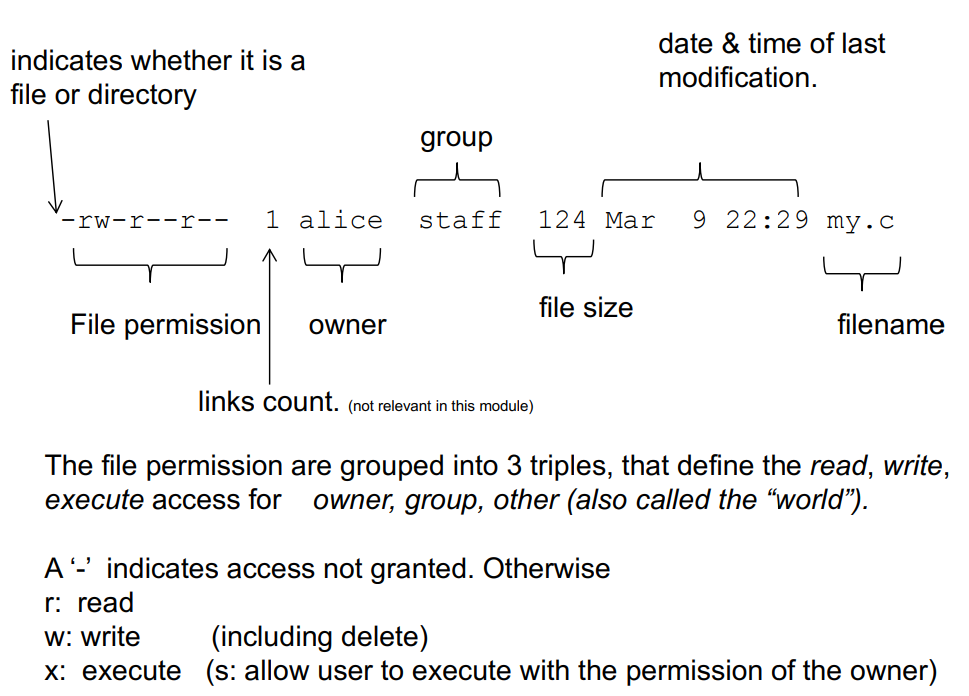
\includegraphics[width=8.5cm, height=5.5cm]{images/unixfilesystempermission.png}
\begin{itemize}[noitemsep,wide=0pt, leftmargin=\dimexpr\labelwidth + 2\labelsep\relax]
    \item Principals are user-identities (UIDs) and group-identities (GIDs).
    \item Information of the user accounts are stored in the “password” file
    \begin{itemize}[noitemsep,wide=0pt, leftmargin=\dimexpr\labelwidth + 2\labelsep\relax]
        \item The file is made world-readable because some information in /etc/passwd is
        needed by non-root program. In earlier version of Unix, the “*” in the file was the
        hashed password H(pw), where H() is some cryptographic hash, and pw the
        password of the user. Hence, previously all users can see the hashed passwords
        of others.
        \item The file is made world-readable because some information in /etc/passwd is
        needed by non-root program. In earlier version of Unix, the “*” in the file was the
        hashed password H(pw), where H() is some cryptographic hash, and pw the
        password of the user. Hence, previously all users can see the hashed passwords
        of others.
    \end{itemize}
    \item \verb|superuser (root)|: A special user is the superuser, with UID 0 and usually with the username root.
    All security checks are turned off for root.
\end{itemize}

\subsubsection*{Checking for file access}
The objects are files. Recall that each file is associated with a 9-bit permission.
Each file is owned by a user, and a group. The owner of a file, or superuser can change the permission bits.
\begin{itemize}[noitemsep,wide=0pt, leftmargin=\dimexpr\labelwidth + 2\labelsep\relax]
    \item If the user is the owner, the permission bits for \textbf{owner} decide the access rights
    \item If the user is not the owner, but the user’s group (GID) owns the file, the permission bits for
    \textbf{group} decide the access rights.
    \item If the user is not the owner, nor member of the group that own the file, then the permission
    bits for \textbf{other} decide.
\end{itemize}

\subsection*{Controlled Invocation \& privilege elevation}
Some sensitive resources (such as network port 0 to 1023, printer) should be
accessible only by the superuser. However, users sometime need those resources.
\begin{itemize}[noitemsep,wide=0pt, leftmargin=\dimexpr\labelwidth + 2\labelsep\relax]
    \item The system provides a predefined set of applications that have access to F.
    \item These application is granted “elevated privilege” so that they can freely access
    the file, and any user can invoke the application. Now, any user can access F via
    the application.
    \item The programmer who write the application bear the responsibility to make sure
    that the application only performed intended limited operation. In other words,
    the user stay within the planned boundary when using the application.
\end{itemize}

\subsubsection*{With Controlled Escalation}
\includegraphics*[width=8.5cm]{images/controlescalation.png}

\subsubsection*{Bridges with Elevated Privilege }
\includegraphics*[width=8.5cm]{images/bridgeselevated.png}
\begin{itemize}[noitemsep,wide=0pt, leftmargin=\dimexpr\labelwidth + 2\labelsep\relax]
    \item “Bridge” is not implemented correctly and contains exploitable
    vulnerabilities. 
    \item In some vulnerabilities, an attacker can trick the bridge to perform
    “illegal” operations not expected by the programmer/designer. This would have
    serious implication, since the process is now running with “elevated privilege”.
    \item Known as \textbf{Privilege escalataion}
\end{itemize}
\includegraphics*[width=8.5cm]{images/maliciousprivilegeescalation.png}

\subsection*{Controlled Invocation in Unix}
A process has an identification (PID). New process can be created by
executing a file or by “forking” an existing process, and associated by \textbf{Real UID} and \textbf{Effective UID}.
\begin{itemize}[noitemsep,wide=0pt, leftmargin=\dimexpr\labelwidth + 2\labelsep\relax]
    \item \textbf{Real UID:} inherited from the user who invokes the process. For e.g. if
    the user is \verb|alice|, then the real UID is \verb|alice|.
    \item \textbf{Effective UID:} Processes can be created by executing a file. Each executable file has a SUID
    flag. 
    \begin{itemize}[noitemsep,wide=0pt, leftmargin=\dimexpr\labelwidth + 2\labelsep\relax]
        \item If the Set User ID (SUID) is disabled (the permission will be displayed as “x”),
        then the process’ \textbf{effective UID} is same as \textit{real UID}.
        \item If the Set User ID (SUID) is enabled (the permission will be displayed as “s”), then
        the process’ \textbf{effective UID} is inherited from the UID of the \textit{file’s owner}. 
    \end{itemize}
    \item When process wants to access a file, the \textbf{effective UID} of the process is treated as
    the “subject” and checked against the file permission to decide if it is granted or denied access.
\end{itemize}
\includegraphics*[width=8.5cm]{images/suidexample.png}

\subsubsection*{Need temp access to root file}
\begin{itemize}[noitemsep,wide=0pt, leftmargin=\dimexpr\labelwidth + 2\labelsep\relax]
    \item Create an executable file \verb|editprofile| owned by \verb|root|: \verb|-r-sr-xr-x 1 root staff 6 Mar 18 08:00 editprofile|
    \item The program is made world-executable so that \textit{any} user can execute.
    \item Furthermore, the permission is set to be “s”: when it is executed, its effective UID will be “root”
    \item Now, if \verb|alice| executes the file, the process’ real UID is \verb|alice|, but its \textbf{effective UID} is \verb|root|.
    Following the checking rule, this process can now read/write the file \verb|employee.txt|.
    
\end{itemize}

\subsubsection*{Elevated Privilege}
\begin{itemize}[noitemsep,wide=0pt, leftmargin=\dimexpr\labelwidth + 2\labelsep\relax]
    \item In this example, the process editprofile is temporary elevated to
    superuser (i.e. root), so that it can access sensitive data. We can view
    the elevated process as the interfaces where a user can access the
    “sensitive” information.
    \begin{itemize}[noitemsep,wide=0pt, leftmargin=\dimexpr\labelwidth + 2\labelsep\relax]
        \item They are the predefined “bridges” for the user to access data.
        \item The “bridge” can only be built by the root.
    \end{itemize}
    \item These bridges solve the problem. However, it is important that these
    “bridges” are \underline{correctly implemented} and do not leak more than required.
\end{itemize}

\end{multicols*}

\end{document}